\documentclass [a4paper, twoside] {book}

\usepackage{amsmath}
\usepackage[utf8]{inputenc}
\usepackage[italian]{babel}
\usepackage{csquotes}
\usepackage{array}
\usepackage{color}
\usepackage{colortbl}
\usepackage{graphicx}
\usepackage{multirow}
\usepackage{siunitx}
\usepackage{hyperref}
\hypersetup{colorlinks=true,
	%% linkcolor=cernblue,
	%% anchorcolor=cernblue,
	%% citecolor=cernblue,
	%% urlcolor=cernblue,
	%% plainpages=false,
	%% pagebackref=true,
  pdftitle={Appunti di Istituzioni di Fisica Applicata},
}

\usepackage{microtype}
\usepackage{listings}
\usepackage{adjustbox}
\usepackage{verbatim}
\usepackage{float}
\usepackage{mathrsfs}
\usepackage{titling}
\usepackage{etoolbox}

\usepackage[
            hyperref=true,
            clearlang=true,
            url=true,
            isbn=true,
            arxiv=abs,
            hyperref=true,
            backref=true,
            sorting=nyt,
%            style=alphabetic,
            style=ieee-alphabetic,
%            style=authoryear,
%            style=apa,
            citereset=chapter,
            maxcitenames=3,
            maxbibnames=100,
            block=space,
%            backend=bibtexu
            backend=bibtex
]{biblatex}
\addbibresource{bibliografia.bib}

%% \usepackage[a4paper,top= 3cm,bottom= 2cm,left= 2cm,right= 2cm]{geometry}
\usepackage[a4paper]{geometry}
\newcommand{\subtitle}[1]{%
  \posttitle{%
    \par\end{center}
    \begin{center}\large#1\end{center}
    \vskip0.5em}%
}

\usepackage[acronym,nomain]{glossaries}
%\gls per gli acronimi
\def\acro#1{\gls{#1}} %ridefinito in \acro

% !TEX root = main.tex

\hyphenation{cal-led}
\hyphenation{of-ten}
%\hyphenation{par-ti-cles}
\hyphenation{con-cen-tra-ted}
\hyphenation{cal-cu-la-tion}
\hyphenation{de-ex-ci-ta-tion}
\hyphenation{mul-ti-ple}
\hyphenation{Cou-lomb}
\hyphenation{Scat-ter-ing}
\hyphenation{main-ly}
%\hyphenation{ro-ta-tio-nal}
\hyphenation{ca-sca-de}
\hyphenation{Brems-strah-lung}
%\hyphenation{proj-ec-ti-le}

%\glsreset{<label>} to reset a label
%\glsresetall reset all
%\acrlong{<label>} to write the extended
%\acrfull{<label>} to write extended and short even if it is not the first time
%\acrshort{<label>} to write the abbreviation

\newacronym{geant}{Geant4}{GEometry ANd Tracking}
\newacronym{fluka}{FLUKA}{FLUktuierende KAskade or Fluctuating Cascade}
\newacronym{mc}{MC}{Monte Carlo}
\newacronym{dna}{DNA}{DeoxyriboNucleic acid}
\newacronym{let}{LET}{Linear Energy Transfer}
\newacronym{rbe}{RBE}{Relative Biological Effectiveness}
\newacronym{nist}{NIST}{National Institute of Standards and Technology}
\newacronym{ginc}{GINC}{Generalised Intra-Nuclear Cascade}
\newacronym{dpm}{DPM}{Dual Parton Model}
\newacronym{dpmjet}{DPMJET}{Dual Parton Model and Jets}
\newacronym{peanut}{PEANUT}{Pre-Equilibrium Approach to NUclear Thermalization}
\newacronym{ensdf}{ENSDF}{Evaluated Nuclear Structure Data File}
\newacronym{bme}{BME}{Boltzmann Master Equation}
\newacronym{rqmd}{RQMD}{Relativistic Quantum Molecular Dynamics}
\newacronym{gdh}{GDH}{Geometry Dependent Hybrid Model}
\newacronym{cnao}{CNAO}{Centro Nazionale di Adroterapia Oncologica}
\newacronym{ptc}{PTC}{Particle Therapy Center}
\newacronym{hit}{HIT}{Heidelberg Ion Beam Therapy Center}
\newacronym{pet}{PET}{Positron Emission Tomography}
\newacronym{ssd}{SSD}{Silicon Strip Detector}


\title{Appunti di Istituzioni di Fisica Applicata}
\subtitle{Dalle lezioni del prof. Riccardo Faccini}
\author{Manuel Loparco}

\begin{document}
\maketitle
\addcontentsline{toc}{chapter}{Appunti di Istituzioni di Fisica Applicata}

\tableofcontents
\addcontentsline{toc}{chapter}{Indice}

\mainmatter

% !TEX root = main.tex

\chapter{Introduzione ed esempi di applicazioni}

Le applicazioni della fisica delle particelle elementari si basano sull'introduzione di radiazione o materiale radiattivo nell'oggetto in studio. In particolare, nel caso medico, l'oggetto in esame è il paziente e la radiazione può uscire da esso (diagnostica), o interagire al suo interno per fini terapeutici (radioterapia).
Verranno considerate radiazioni di tipo $\beta-$ e $\alpha$, che comportano un rilascio di energia locale, radiazioni di tipo $\beta+$ in cui il positrone creato riemette energia sottoforma di fotoni, e radiazione puramente elettromagnetica.\\
Per un'introduzione approfondita alla fisica medica e alla fisica nucleare consultare nella bibliografia le fonti \cite{ENMP} \cite{NMP}, \cite{CLA}, \cite{Corvisiero3}, \cite{Nutshell}.\\

Si riporta qui una vetrina di possibili applicazioni della fisica della radiazione che saranno utilizzate nel seguito per esemplificare gli argomenti di fisica che si andranno a studiare.

\section{Diagnostica}

La diagnostica può essere \emph{morfologica} se dà informazioni sulla morfologia del corpo (densità, presenza di masse anomale). Esempi sono la CT e la radiografia 2D, che usano i raggi X.\\
Oppure può essere \emph{funzionale} se dà anche informazioni di tipo metabolico. Esempi sono PET e SPECT, che usano decadimenti $\beta+$ che portano a produzione di coppie di fotoni.
La diagnostica funzionale si basa sulla somministrazione di radiofarmaci, ovvero sostanze che vengono assorbite dall'organo di interesse per \emph{metabolismo} o \emph{recettorialità}. Si parla di assorbimento tramite metabolismo quando vengono sfruttate proprietà fisiche dell'organo in esame, come la presenza di membrane che possono essere superate solo da sostanze di dimensioni ridotte. L'assorbimento tramite recettorialità invece si basa sulle proprietà chimiche dei recettori presenti nelle membrane dei tessuti di interesse. Radiofarmaci specifici, infatti, possono simulare le caratteristiche chimiche di uno specifico ligando, reagendo al suo posto con i recettori nelle membrane cellulari dei tessuti dell'organo in esame, mantenendo così la sostanza radioattiva in vicinanza delle cellule che si vogliono esaminare.

 Esempi pratici:
\begin{itemize}
\item Single Photon Emission Computed Tomography (SPECT). Fa utilizzo di $^{131}\text{I}$ o $^{99m}\text{Tc}$. Ad esempio il Tecnezio viene rapidamente smaltito nei reni. Una volta lì esso emette raggi $\gamma$ di $140 keV$ di energia. Con una tecnica chiamata tomografia è possibile dedurne la posizione e ricostruire il metabolismo dei reni.
\item Positron Emission Tomography (PET). Tipicamente fa uso di $^{18}\text{F}$ legato a molecole di zucchero che vengono assorbite dal cervello e da tumori sia primari che metastatici. Permette anche di determinare lo stadio del tumore, e nel particolare se durante la terapia il tumore sta recedendo o meno. Il funzionamento della PET si basa sul fatto che l'isotopo del Fluoro $^{18}\text{F}$ decade $\beta+$. I positroni che vengono emessi da tale processo, interagendo con gli elettroni nelle vicinanze, possono o annichilire in volo o formare positronio. In entrambi i casi vengono emesse coppie di fotoni $\gamma$ che possono essere sfruttate per ricostruire con tecniche tomografiche la posizione dell'isotopo del Fluoro e di conseguenza dei tessuti che lo hanno assorbito.
\item Chirurgia Radio-Guidata. Evidenzia i tumori per aiutarsi nella loro rimozione. Si usa spesso per i linfonodi. L'ultima frontiera è l'utilizzo di nuclidi che decadono $\beta-$.
\end{itemize}

Approfondimenti sulla PET nella bibliografia: \cite{PET1} \cite{PET2}.\\

Approfondimento sulla CT: \cite{CT}\\

Approfondimenti sulla chirurgia radioguidata: \cite{Radiosurgery} \cite{Intraoperative_probes}.

\section{Radioterapia}

La Radioterapia si basa sulla distruzione del meccanismo riproduttivo del tumore, ovvero del DNA. Esso va rotto in almeno due punti o si potrà riprodurre. La radioterapia convenzionale, ottenuta irraggiando il paziente con fotoni o elettroni, non ha energia sufficiente a rompere direttamente il DNA. Piuttosto crea radicali liberi rompendo molecole d'acqua che poi intossicano la cellula tumorale. \`E una sorta di chemioterapia localizzata. Studieremo la differenza nel rilascio di energia tra fotoni e adroni e perché è più conveniente usare questi ultimi.\\

Altri due tipi di radioterapia sono la terapia radiometabolica che si basa sulla distruzione direttamente dall'interno di un tumore sfruttando un radiofarmaco metabolico e la brachiterapia, che consiste nell'applicazione locale sulla pelle di pomate formate da nuclei radioattivi.\\

Approfondimenti sull'adroterapia: \cite{Rossi} \cite{Braccini} \cite{ADRO} \cite{Boron} \cite{Acceleratori_adronterapia} \cite{LINAC}\\

Approfondimento sulla brachioterapia: \cite{Brachioterapia}

\section{Teragnostica}

Con il termine 'teragnostica' si indicano tutte quelle tecniche che tentano di attuare una terapia sul paziente estraendo allo stesso tempo informazioni sulla morfologia e la posizione dei tumori da attaccare. 
Si fa con elementi che emettono contemporaneamente beta- e gamma. Questi ad esempio sono $^{177}\text{Lu}$ e $^{90}\text{Y}$ con $^{68}\text{Ga}$.

\section{Beni Culturali - Ion Beam Analysis (IBA)}

Tecniche analoghe possono essere applicate ai beni culturali. Analizzando l'emissione di radioattività dell'oggetto in esame ad esempio si possono dedurre le seguenti caratteristiche: 

\begin{itemize}
\item Datazione
\item Composizione superficiale
\item Ricerca di contraffatti
\item Corrosione
\item Provenienza
\end{itemize}

Le tecniche di analisi fanno parte della famiglia detta Ion Beam Analysis (IBA), il cui principio base consiste nel bombardare l'oggetto con ioni (generalmente protoni o particelle alfa) e studiare le conseguenze. Questa famiglia contiene al suo interno le seguenti tecniche:
\begin{itemize}
\item Proton Induced X-rays Emission (PIXE), Bombardamento non invasivo di protoni che provocano l'emissione di uno spettro nella regione dei raggi X.
\item Rutherford Backscattering Spectroscopy (RBS), Utile per campioni sottili formati da elementi pesanti. Si analizza la distribuzione dell'angolo con cui le particelle inviate scatterano all'indietro.
\item Elastic Recoil Detection analysis (ERD), Simile al precedente ma funziona per bersagli formati da elementi leggeri.
\item Proton Induced Gamma-rays Emission (PIGE), Come la PIXE ma funziona per elementi leggeri, e si basa sull'emissione di uno spettro nella regione dei raggi gamma.
\end{itemize}

Un'altra tecnica di analisi dei beni culturali che però non si basa su bombardamento di ioni è la X-Ray Fluorescence (XRF), che consiste nel bombardamento del campione con raggi X e nell'analisi della radiazione riemessa per fluorescenza.\\

Approfondimento sui beni culturali: \cite{Cultural}


\section{Datazione col $^{14}\text{C}$}

In natura il Carbonio esiste in tre isotopi, di cui due stabili $^{12}\text{C}$, $^{13}\text{C}$ ed uno radioattivo, $^{14}\text{C}$ con vita media $\tau=8267y$.
La concentrazione media di $^{14}\text{C}$ nell'atmosfera terrestre tende a rimanere costante grazie al continuo flusso di raggi cosmici che vi incide. Infatti  componenti secondari dei raggi cosmici sono i neutroni, che quando si scontrano con i due isotopi stabili del carbonio portano alla produzione di $^{14}\text{C}$.
Nell'atmosfera dunque il rapporto tra numero di isotopi radoattivi e stabili è costante, intorno a $10^{-12}$. \\
Finché un organismo è vivo, esso attua processi di respirazione, fotosintesi o si nutre di altri esseri viventi. In tal modo scambia carbonio con l'atmosfera, mantenendo costante il rapporto tra isotopi del carbonio radioattivi e stabili nel suo corpo. Dopo la sua morte, tali processi cessano. Il carbonio radioattivo decade senza essere riacquistato dall'atmosfera, e dunque il rapporto tra isotopi radioattivi e stabili comincia a scendere in maniera prevedibile.\\
Studiando un organismo deceduto, dunque, si può dedurre in quale periodo storico esso viveva.

\section{Neutroni}

Dato un certo elemento la sua probabilità di interazione con i raggi X è inversamente proporzionale alla sua probabilità di interazione con un neutrone. Allora i neutroni servono laddove i raggi X non riescono a ricavare informazioni sufficienti.
Ad esempio i neutroni vengono assorbiti subito dall'acqua, rendendoli utili per tomografie in cui si voglia evidenziare la presenza di acqua (motori). \\
Approfondimenti sui neutroni: \cite{Corvisiero} \cite{Assay}



% !TEX root = main.tex

\chapter{Unità Naturali}

Portare avanti nelle epressioni matematiche tutte le costanti fondamentali può essere pesante. Pertanto si sceglie di non considerarle quando considerazioni dimensionali permettono di ricostruire quali costanti vanno inserite a posteriori. E' questo il caso della meccanica quantistica e relativistica, dove risulta conveniente porre:

\begin{equation}
c=\hbar=1
\end{equation}

Visto che poi è possibile ricostruire quali sono le potenze mancanti di queste costanti all'interno delle formule.

Nella tabella 2.1 sono riassunti i valori di tali costanti nelle più comuni unità di misura. Conoscendo tali valori è possibile effettuare i calcoli a posteriori.
Le unità di misura ottenute in questo modo, unitamente alla definizione della costante di struttura fine $\alpha_{em}=\frac{e^2}{4\pi\epsilon_0\hbar c}\sim\frac{1}{137}$ che, poste $c=\hbar=1$ diventa $\alpha_{em}=\frac{e^2}{4\pi\epsilon_0}$, costituiscono il sistema di unità naturali.

\begin{table}
\center
\begin{tabular}{|l|l|l|}
\hline
                                                            & Dimensioni                                             & Misura                           \\ \hline
\multicolumn{1}{|c|}{\multirow{3}{*}{$\hbar$}} & \multirow{3}{*}{energia$\cdot$ tempo}     & $1,035 \cdot 10^{-34} J\cdot s$  \\ \cline{3-3} 
\multicolumn{1}{|c|}{}                                      &                                                        & $6,5 \cdot 10^{-16} eV\cdot s$   \\ \cline{3-3} 
\multicolumn{1}{|c|}{}                                      &                                                        & $6,5 \cdot 10^{-13} MeV\cdot ns$ \\ \hline
\multirow{4}{*}{c}                                          & \multirow{4}{*}{posizione/tempo}                       & $3,0\cdot10^8 m/s$               \\ \cline{3-3} 
                                                            &                                                        & $300 km/s$                       \\ \cline{3-3} 
                                                            &                                                        & $\mathbf{30 cm/ns}$              \\ \cline{3-3} 
                                                            &                                                        & $3,0\cdot10^{14} fm/ns$          \\ \hline
\multirow{2}{*}{$\hbar$ c}                     & \multirow{2}{*}{energia$\cdot $posizione} & $3,1\cdot 10^{-26} J\cdot m$     \\ \cline{3-3} 
                                                            &                                                        & $\mathbf{200 MeV \cdot fm}$            \\ \hline
\end{tabular}
\caption{Valori delle costanti $\hbar$ e $c$ nelle più comuni unità di misura}
\end{table}

Il metodo più semplice per convertire le grandezze da unità naturali a sistema internazionale, è porre:

\begin{equation}
Q_{SI}=Q_{UN}\cdot(\hbar c)^m\cdot c^n
\end{equation}

Dove $Q_{UN}$ è una qualsiasi grandezza espressa nel sistema di unità naturali, $Q_{SI}$ è la stessa grandezza espressa nel sistema di unità internazionale e $m$ ed $n$ sono le specifiche potenze che bisogna porre ai termini $\hbar c$ e $c$ affinché le dimensioni della grandezza considerata siano coerenti in entrambi i sistemi di unità di misura.\\
Si consiglia di utilizzare i valori delle costanti espresse in grassetto nella tabella 2.1.

\section{Cinematica e Dinamica Relativistica}

Il sistema di unità naturali è specialmente utile perché semplifica le equazioni della relatività ristretta. Nella tabella 2.2 è presente una comparazione di tale equazioni nel sistema di unità internazionale e in quello di unità naturali

\begin{table}
\centering
\begin{tabular}{|l|l|}\hline
SI & UN \\ \hline
$\beta=\frac{v}{c}$   & $\beta=v$   \\ \hline
$E=\sqrt{p^2c^2+m^2c^4}$   &   $E=\sqrt{p^2+m^2}$ \\ \hline
$p=m\beta\gamma c$   &  $p=m\beta\gamma$  \\ \hline
$T=E-mc^2$   &  $T=E-m$  \\ \hline 
   &  $\beta=\frac{p}{E}$  \\ \hline
   &  \\ \hline
\end{tabular}
\label{equazioni}
\caption{Confronto delle equazioni di cinematica relativistica nei due sistemi di unità di misura}
\end{table}

\subsection{Esempi ed Applicazioni}

\emph{Un elettrone ha quantità di moto $p_{UN}=1 MeV/c$. Quale è la sua quantità di moto espressa nel sistema internazionale?}

Ricordando la conversione $1 eV=1,6\cdot10^{-19} J$ e il valore della velocità della luce $c=3\cdot 10^8 m/s$, otteniamo:

\begin{equation}
p_{SI}=p_{UN}\cdot\frac{1,6\cdot10^{-19}\cdot10^6}{3\cdot10^8}=5\cdot10^{-22}kg\cdot m/s
\end{equation}

\emph{Qual è l'energia elettrostatica di un elettrone a distanza $d=0,5$\AA da un nucleo di carbonio, trascurando lo schermaggio prodotto dagli altri elettroni?}

Ricordando l'espressione per l'energia potenziale elettrostatica per un sistema di due cariche puntiformi abbiamo

\begin{equation}
U=\frac{Ze^2}{4\pi\epsilon_0d}=\frac{Z\alpha_{UN}}{d}
\end{equation}

Dove $\alpha_{UN}=\frac{e^2}{4\pi\epsilon_0}\sim\frac{1}{137}$ è detta costante di struttura fine ed è adimensionale: non dipende dunque dal sistema di unità di misura scelto. Facendo un'analisi dimensionale ora decidiamo quali potenze di $\hbar c$ e $c$ vanno aggiunte.

A sinistra abbiamo un'energia, a destra l'inverso di una lunghezza.

\begin{equation}
E=\frac{([\hbar c])^m \cdot [c]^n}{L}=(E\cdot L)^m\left(\frac{L}{T}\right)^n\cdot L^{-1}
\end{equation}

Da cui si ricava che necessariamente $m=1$ e $n=0$. Ovvero:

\begin{equation}
U=\frac{Z\alpha\hbar c}{d}=\frac{6\cdot\frac{1}{137}\cdot200MeV\cdot fm}{5\cdot 10^4 fm}=175eV
\end{equation}

Dove ci siamo ricordati che 1\AA$=10^{-10}m$ e $1 fm=10^{-15}m$.

Esercizi ulteriori:

\begin{itemize}
\item \emph{Qual è l'energia cinetica di un nucleo di Elio con impulso $p=50MeV/c$?}
\item \emph{Qual è il raggio dell'orbita di un protone con energia cinetica $T=10MeV$ immerso in un campo magnetico di modulo $B=0,5 T$?}
\item \emph{Quali sono la $\beta$ e $\beta\gamma$ di un elettrone accelerato da $1 MV$?}
\end{itemize}



% !TEX root = main.tex

\chapter{Interazioni tra Radiazione e Materia}

In questo capitolo studieremo come interagiscono con la materia ioni, elettroni, positroni, fotoni, neutroni.

\section{Interazioni Ioni-Materia}

\begin{figure}
\centering
	%% %% 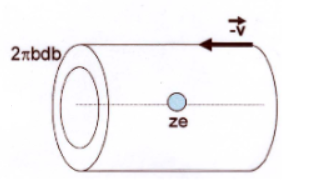
\includegraphics[keepaspectratio]{rutherford.png}
	\caption{Applicazione del teorema di Gauss nel sistema di riferimento dello ione}
	\label{fig:rutherford}
\end{figure}


Ai regimi di energia che interessano a noi gli ioni interagiscono prevalentemente con gli elettroni della materia su cui incidono, potenzialmente ionizzandola. Si usano come ioni proiettili atomi completamente ionizzati quali $H^+$, $He^{2+}$ e $C^{6+}$.
Inoltre l'energia dello ione è dell'ordine del MeV, mentre quella dell'elettrone ordine eV, dunque nella schematizzazione che segue considereremo fermo l'elettrone.
Siccome lo ione è molto più massivo dell'elettrone possiamo metterci nel suo sistema di riferimento e considerarlo imperturbato nel corso dell'interazione. 

\begin{equation}
\Delta p_e=\int Fdt = e\int Edt = \frac {e}{v}\int E \mathrm{d}x
\end{equation}

Prendendo un cilindro immaginario intorno allo ione ed applicando il teorema di Gauss ottengo

\begin{equation}
\Phi(E)=2\pi b \int E \mathrm{d}x =\frac{Ze}{\epsilon_0}
\end{equation}

Dove $b$ è il raggio di base del cilindro.\\
Dalla precedente equazione si ricava:

\begin{equation}
\int E \mathrm{d}x= \frac{Ze}{2\pi b \epsilon_0}
\end{equation}

Sostituendo nell'espressione per la variazione della quantità di moto dell'elettrone ottengo:

\begin{equation}
\Delta p_e=\frac{Ze^2}{2\pi\epsilon_0vb}
\end{equation}

Da cui l'energia cinetica totale trasferita da ione a elettrone è:

\begin{equation}
\Delta K_{I,e}=\frac{\Delta p_e^2}{2m_e}=(\frac{Ze^2}{2\pi\epsilon_0vb})^2\frac{1}{2m_e}
\end{equation}

Verifichiamo ora che le approssimazioni fatte siano ragionevoli. Prendiamo ad esempio uno ione idrogeno incidente con impulso iniziale di $100 MeV/c$. Per esso $E\simeq m$ dunque $\beta\simeq\frac{p}{m}=0,1$.

\begin{equation}
 |\Delta p_I|=|\Delta p_e|=\frac{Ze^2}{2\pi\epsilon_0vb}=\frac{2Z\alpha}{\beta b}\cdot(\hbar c)^mc^n  
\end{equation}

Dall'equazione $p=\frac{E}{c}$ per l'impulso di una particella non massiva sappiamo che le dimensioni dell'impulso sono $[p]=\frac{E\cdot T}{L}$. Le dimensioni corrette si ottengono nell'equazione precedente scegliendo quindi $m=1$ e $n=-1$.

\begin{equation}
|\Delta p_I|=\frac{2\cdot 200 MeV\cdot fm}{137 \cdot 0,1 \cdot c \cdot b}
\end{equation}

A noi interessa capire per quali valori di $b$ vale la approssimazione $\frac{\Delta p_I}{p_I}<<1$. 
Con i dati che abbiamo noi ciò si traduce in $\Delta p_I<<100 MeV/c$ ovvero 

\begin{equation}
\frac{29 fm}{b}<<100
\end{equation}

Che si traduce come condizione su $b$ in:

\begin{equation}
b>>0,3 fm
\end{equation}

E ciò si verifica praticamente sempre. Ovvero lo ione per essere perturbato nel suo moto dovrebbe avvicinarsi a meno di $0,3 fm$ dal nucleo, cosa altamente improbabile.

\emph{Nota: il trasferimento di impulso è inversamente proporzionale alla velocità dello ione! Infatti più esso è lento, più tempo trascorre vicino all'elettrone, trasferendogli impulso.}

Bibliografia: \cite{Longo}

\section{Bethe-Block}

La formula di Bethe-Block descrive la perdita di energia per unità di spazio percorso per una particella massiva carica che fa ionizzazione in un materiale. Tale formula si dimostra\footnote{\texttt{https://userswww.pd.infn.it/~carlin/riv/Slides/parte1.pdf}} essere:

\begin{equation}
-\frac{dE}{dx}=4\pi N_A\frac{Z\rho}{A}r_e^2m_ec^2\frac{z^2}{\beta^2}(\ln\frac{2m_ec^2\beta^2\gamma^2}{I}-\beta^2-\frac{\delta(\gamma)}{2})
\end{equation}

Nel range di energie che interessano a noi ($\beta\gamma<2$) la funzione è approssimabile nella formula $\frac{1}{\beta^2}$ ovvero all'aumentare della velocità la perdita di energia scende con il suo quadrato. Come avevamo visto dalle considerazioni nel paragrafo precedente se lo ione incidente è più lento, perderà più energia nell'unità di percorso. Al di là del tipo di materiale in cui sto incidendo, in generale, per $\beta\gamma$ dell'ordine dell'unità ho che $-\frac{1}{\rho}\frac{dE}{dx}\simeq2MeV g^{-1}cm^{2}$.
Il fatto che lavoriamo ad energie più basse si vede perché imponendo $\beta\gamma=3$ si ottiene un energia cinetica dell'ordine dei $5 GeV$, molto maggiore di quelle effettivamente usate in medicina.

\begin{figure}
\centering
	%% 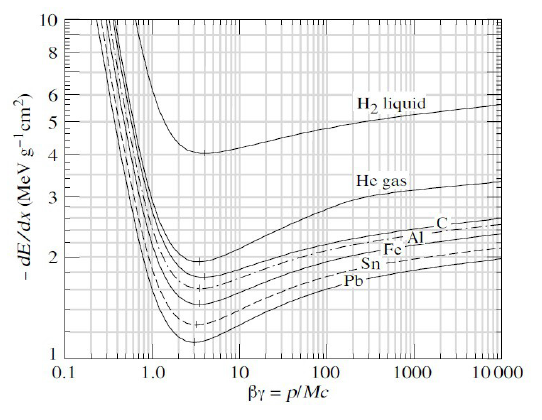
\includegraphics[width=10cm, keepaspectratio]{bethe.png}
	\caption{Grafico della formula di Bethe-Block. Si osserva il primo tratto di discesa in cui domina il termine $\frac{1}{\beta^2}$, il minimo a $\beta\gamma=2m_0c^2$ e il seguente tratto di risalita.}
	\label{fig:bethe}
\end{figure}



\newpage

\section{Stopping Power e Linear Energy Transfer (LET)}

Abbiamo visto prima l'andamento della Bethe Block e l'intervallo di nostro interesse. Fissata una velocità iniziale, il moto della particella in esame attraverso un certo materiale può solo rallentare. Ovvero la particella può solo muoversi a sinistra nel grafico e quindi rimarrà sempre nel regime $\frac{1}{\beta^2}$. In pratica con lo svolgersi del processo la particella diminuirà $\beta\gamma$ e aumenterà $\frac{dE}{dx}$, fino ad un massimo che corrisponderà al range totale della particella, dopo il quale essa ha perso tutta l'energia. L'integrale di $\frac{dE}{dx}$ da 0 al range deve restituire dunque l'energia iniziale della particella. 
Questo $\frac{dE}{dx}$ rappresenta lo stopping power, ovvero l'energia rilasciata dalla particella. Essa non sempre coincide con l'energia assorbita dal paziente. La quantità che misura l'energia assorbita dal paziente è il LET. La prima differenza quantitativa tra le due grandezze è che il LET va come $\frac{1}{\beta^{2*0,82}}$ e la formula empirica che lo descrive (valida nel range di energie trattate nella fisica medica) è:

\begin{equation}
LET=\frac{L_0Z^2}{(K/m)^{0,82}} \qquad \qquad L_0(acqua)=0,12 \frac{keV}{\mu m}
\end{equation}

Passiamo al calcolo del Range \cite{Amaldi}:

\begin{equation}
R=\int_{K_0}^0 \frac{dK}{-|{\frac{dE}{dx}|}} =\int_0^{K_0} \frac{dK}{LET} = \int_0^{K_0} \frac{dK (K/m)^{0,82}}{L_0Z^2}  
\end{equation}

\begin{equation}
R(K)=R^*\frac{A}{Z^2}(K/m)^{1,82} \qquad \qquad R^* = 425 cm
\end{equation}

\emph{Nota: queste considerazioni valgono per $K/m<$0,4. Nel caso di protoni ciò si traduce in $K<400 MeV$.}

Questa formula per $R$ può essere intesa come funzione di $K$. Ovvero esprime il cammino che resta alla particella in esame se ha energia cinetica $K$. Posso anche esprimere il $LET$ in funzione del cammino che resta: basta invertire la relazione tra $R$ e $K$ e sostituire nella formula del LET. Si ottiene:

\begin{equation}
LET(R)=L_0Z^{1,1}A^{0,45}(R^*/R)^{0,45}
\end{equation}

Ora, considerando che $R$ è il cammino restante alla particella e $x=R_0-R$ e la posizione reale, l'equazione precedente viene riformulata:

\begin{equation}
LET(x)=L_0Z^{1,1}A^{0,45}(\frac{R^*}{R_0-x})^{0,45}
\end{equation}

\textbf{Prima Esercitazione}

\emph{Graficare il range in funzione dell'energia cinetica e il LET in funzione della posizione per protoni, particelle alfa e nuclei di carbonio in acqua.}

L'espressione analitica di LET(x) presenta un asintoto. Nella realtà esso viene scavalcato, perché il fascio di particelle incidenti ha sempre un'incertezza sulla sua energia e sulla sua distribuzione spaziale. Solo un fascio puramente monocromatico avrebbe un andamento asintotico. 

Il massimo assunto di LET(x) deve essere di $20 eV/mm$ per distruggere direttamente il DNA tumorale. Se si vuole solo creazione di radicali liberi bastano energie anche minori.

L'adroterapia è convenzionalmente a basso LET, col solo obiettivo di creare radicali liberi. 

Il plot reale dell'andamento di LET(x) è detto curva di Bragg. Confrontando la curva di Bragg di un protone con quella di un nucleo di carbonio facciamo le seguenti osservazioni:

\begin{itemize}
\item Il picco di Bragg degli ioni carbonio è più stretto e più alto di quello dei protoni
\item Il carbonio presenta una coda dopo il picco che risulta pericolosa
\end{itemize}

\begin{figure}
\centering
	%% 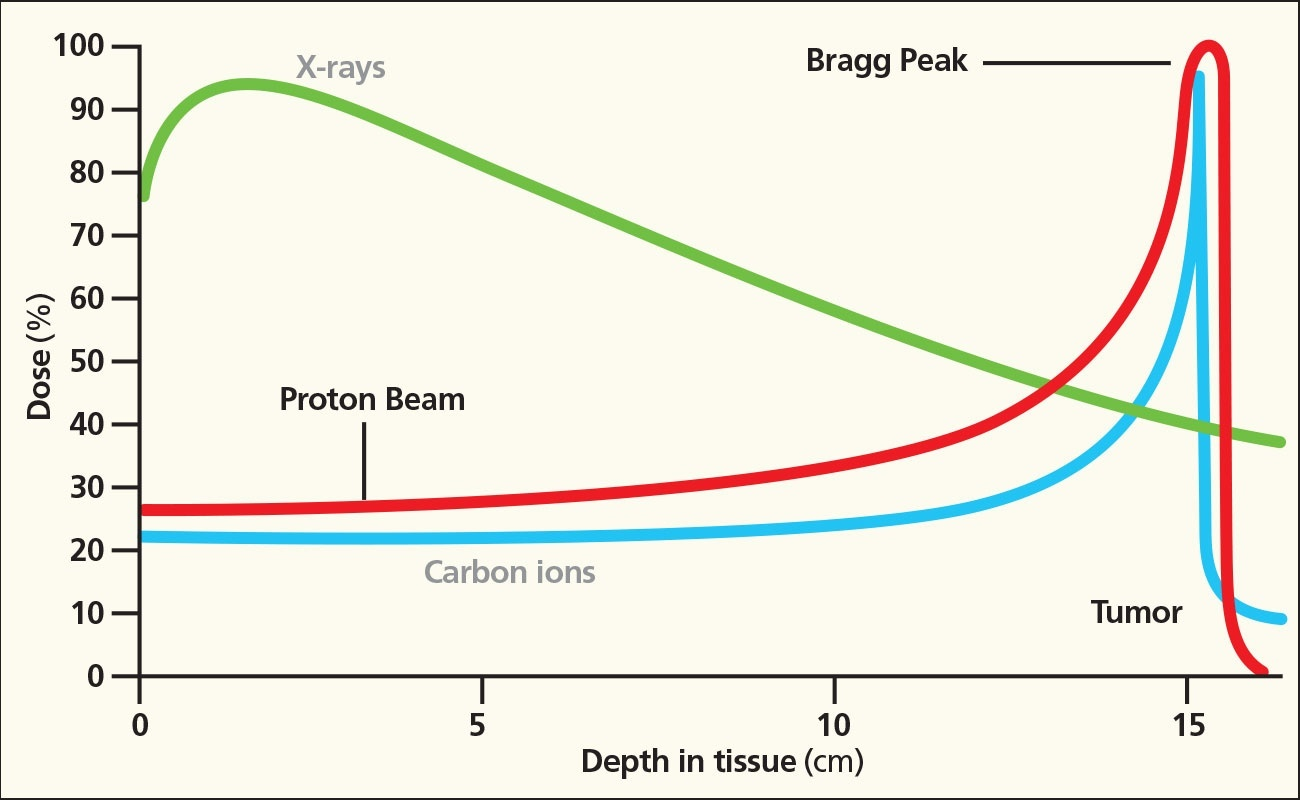
\includegraphics[width=10cm, keepaspectratio]{bragg.jpg}
	\caption{Dose relativa in funzione della penetrazione per fotoni, protoni e carbonio. Il grafico è rappresentativo dell'andamento di LET(x) a meno di una costante. Immagine da scripps.org}
	\label{fig:bragg}
\end{figure}


\section{Scattering Multiplo - Ioni-Nuclei}

Fino ad ora abbiamo osservato il caso in cui lo ione interagisca con gli elettroni del materiale e ci sia un trasferimento di energia per ionizzazione.
Nel caso in cui però lo ione interagisca con il nucleo invece di uno scambio di energia ci sarà una variazione di quantità di moto che si concretizza in una variazione di direzione per lo ione. Esso verrà deviato nel suo percorso. Siccome avvengono tante di queste interazioni si parla di \emph{Scattering Multiplo}. 
Il risultato finale è che un fascio collimato fuoriesce con una distribuzione gaussiana con deviazione standard:

\begin{equation}
\sqrt{\sigma_{\theta}^2}=\frac{z}{\beta p}\sqrt{\frac{x}{X_0}}
\end{equation}

Dove $x$ è lo spessore percorso, $X_0$ una costante del materiale.

\emph{Nota: Il multiple scattering è la vera ragione dello smussamento dell'asintoto di $LET(X)$. Infatti se ad energie diverse corrisponde un angolo finale diverso ciò vuol dire che il range (proiettato su X) è diverso per ogni energia e dunque si spalma intorno al massimo. Da qui anche il motivo per cui il carbonio ha un massimo più definito: subisce meno multiple scattering.}

\begin{figure}
\centering
	%% 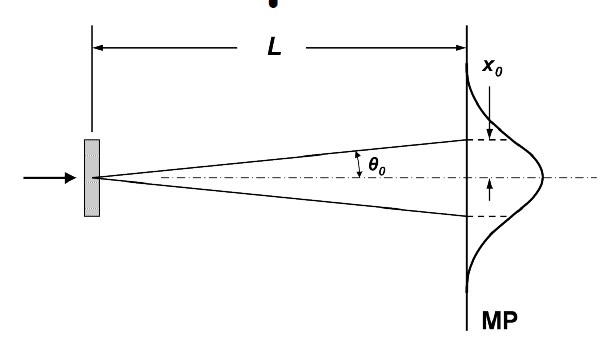
\includegraphics[width=10cm, keepaspectratio]{multiplescattering.png}
	\caption{Rappresentazione dell'effetto del Multiple Scattering. L'angolo in uscita ha una distribuzione di tipo gaussiano.}
	\label{multiplescattering}
\end{figure}

\textbf{Seconda Esperienza}

\begin{itemize}
\item \emph{Stimare CSDA (range reale, non proiettato) e range proiettato in acqua per particelle alfa e protoni con energia cinetica tra $1$ e $10$ $MeV$.}
\item \emph{Stimare la quantità di teflon, ferro e piombo necessarie a fermare particelle alfa e protoni di energie $1$, $5$ e $10$ $MeV$.}
\end{itemize}

\section{Interazioni Elettroni-Materia}

Un elettrone che incide sul bersaglio può interagire fondamentalmente in tre modi. Il primo è per ionizzazione come gli ioni. La formula di Bethe Block va aggiustata per questioni relativistiche e diventa

\begin{equation}
-\frac{dE}{dx}=0,306 N_A\frac{Z\rho}{A}\frac{1}{\beta^2}\ln(\frac{1,16m_ec^2\beta^2}{2I}) MeV/cm\qquad per \beta<0,5
\end{equation}

\begin{equation}
-\frac{dE}{dx}=0,153 N_A\frac{Z\rho}{A}\frac{1}{\beta^2}\ln(\frac{E(E+m_ec^2)^2\beta^2}{2I^2m_ec^2}) MeV/cm \qquad per \beta\simeq 1
\end{equation}

Se invece l'elettrone interagisce con i nuclei del materiale può avvenire multiple scattering (molto più intenso che per gli ioni data la leggerezza degli elettroni) o Brehmsstrahlung. 
Infatti un elettrone che viene deviato nel suo moto da un nucleo, emette radiazione. La potenza dell'emissione è data da:

\begin{equation}
W(\theta)=\frac{q^2a^2sin^2\theta}{4\pi\epsilon_{0}c^3}
\end{equation}

\begin{figure}
\centering
		%% 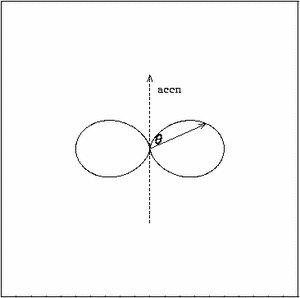
\includegraphics[width=6cm, keepaspectratio]{brehm.png}
		\caption{Andamento dell'energia irradiata in funzione dell'angolo con la direzione del moto}
         \label{brehmtheta}
\end{figure}

Dove $\theta$ è l'angolo tra la direzione del moto dell'elettrone e la direzione della radiazione irradiata.

L'effetto sull'energia dell'elettrone è dato dalla seguente equazione:

\begin{equation}
-\frac{dE}{dx}=\frac{E}{X_0}
\end{equation}

Con soluzione

\begin{equation}
E(x)=E(0)e^{-x/X_0}
\end{equation}

dove 

\begin{equation}
X_0\simeq\frac{A}{N_A Z^2 \rho}\frac{1}{4 \alpha_{em}r_e^2 \ln(\frac{184}{Z^{1/3}})}
\end{equation}

Allo spettro continuo prodotto dalla radiazione di frenamento si possono sommare inoltre delle righe caratteristiche dovute ad un secondo processo: la radiazione di guscio K. 
Questo processo si verifica quando il fotone emesso dall'elettrone frenato ionizza gli atomi del bersaglio colpendo non gli elettroni di valenza ma quelli più vicini al nucleo. Quando ciò succede gli elettroni esterni possono scendere ai livelli più vicini al nucleo emettendo radiazione X. Si parla di $K_{\alpha}$ quando si indica la radiazione emessa da un elettrone che passa da $n=2$ a $n=1$, mentre si parla di $K_{\beta}$ quando si vuole indicare radiazione emessa da un elettrone che scende da $n=3$ a $n=1$. Questa radiazione è monocromatica, pur essendo in origine generata da uno spettro continuo.

Lo spettro totale è mostrato nella figura (\ref{brehmspect})

\begin{figure}
\centering
		%% 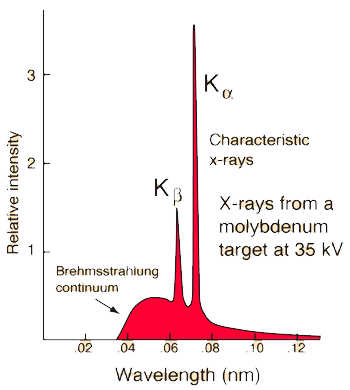
\includegraphics[width=7cm, keepaspectratio]{Spettroxrays.png}
		\caption{Spettro della radiazione risultante, dato da Brehmsstrahlung e radiazione di guscio K}
         \label{brehmspect}
\end{figure}

Notare che la lunghezza d'onda più spostata a sinistra coincide con l'energia iniziale dell'elettrone.

\emph{Nota: per elettroni proiettili la radiazione di frenamento domina sulla ionizzazione solo se $E>\frac{800 MeV}{Z}$. Nel corpo umano $Z\sim6$ dunque la radiazione di frenamento domina come $LET$ solo se $E>133 MeV$ che è enorme per le energie mediche. Quindi nei nostri interessi per gli elettroni nei pazienti domina sempre la ionizzazione.}

A causa dell'intensità del multiple scattering che porta alla dispersione degli elettroni, non ha più senso proiettare il $LET$ sull'asse $x$. La distribuzione viene tutta concentrata all'inizio perché proiettando concentro lì tutte le direzioni diverse da quella $x$.
Questa distribuzione del $LET$ ha un applicazione notevole: utile per i tumori della cute. Si spalma una pomata contenente $^{118}Re$ (\emph{Brachiterapia}\cite{Brachioterapia}) o si spara direttamente con un LINAC sulla zona interessata, che magari è la parete di un organo sensibile da cui è difficile asportare il tumore (Intra Operative Radio Therapy (IORT)\cite{Intraoperative_probes}), ad esempio le pareti dell'aorta.
Per lo spettro completo (Brehmsstrahlung + radiazione caratteristica) guardare la Tesina.
Assumendo un ascissa curvilinea che segue il percorso da multiple scattering degli elettroni e graficando il $LET$ in funzione di tale ascissa osservo un grafico identico a quello del protone proiettato. Tale ascissa curvilinea è detta $CSDA$.

\begin{figure}
\centering
		%% 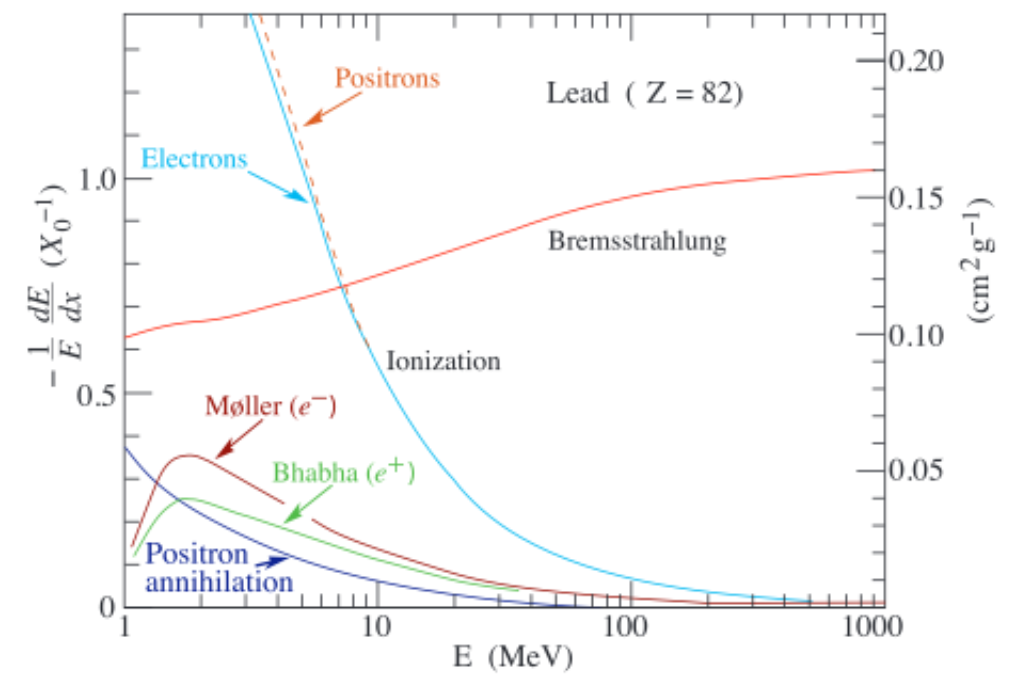
\includegraphics[width=10cm, keepaspectratio]{stoppingpower.png}
		\caption{Confronto dello stopping power per diversi tipi di radiazione nel piombo.}
         \label{stoppingpower}
\end{figure}


\section{Interazioni Fotoni-Materia}


Nelle interazioni tra fotoni e materia la probabilità che un quanto di luce interagisca con la materia in un trattino $\mathrm{d}x$ è effettivamente indipendente dal resto del cammino. Questa probabilità è proporzionale alla larghezza del trattino e dunque si può scrivere la seguente relazione:

\begin{equation}
\mathrm{d}p=\mu \mathrm{d}x
\end{equation}

Dove il coefficiente di proporzionalità $\mu$ viene chiamato coefficiente di assorbimento, e dipende dal tipo di interazione che sta avvenendo, nonché dall'energia del fotone incidente. Il numero di fotoni che vengono assorbiti in un tratto $dx$ allora sarà dato dalla seguente relazione:

\begin{equation}
\mathrm{d}N(x)=-N(x)\mu \mathrm{d}x
\end{equation}

Con soluzione

\begin{equation}
I(x)=I(0)e^{-\mu x}
\label{Intensity}
\end{equation}

Dove si è considerato che l'intensità di un fascio luminoso è proporzionale al numero di fotoni che compongono tale fascio.
In generale si possono avere più interazioni di vario tipo, con diverso coefficiente di assorbimento. Sommando i contributi di tale interazioni si ha che:

\begin{equation}
\mu=\sum \mu_{i}
\end{equation}

Introduciamo ora invece il concetto di sezione d'urto. 
La sezione d'urto è una grandezza prettamente sperimentale. In una schematizzazione classica in cui il fascio incidente incontra una serie di ostacoli che bloccano parte di tale fascio facendone passare il resto, la sezione d'urto rappresenta la superficie ostacolante costituita nel nostro caso dalle molecole del corpo umano. L'equazione differenziale che la definisce è la seguente:

\begin{equation}
\mathrm{d}\Phi(x)=-\sigma_{b}n_{b}\Phi(x)\mathrm{d}x
\end{equation}

Dove $\Phi$ è il flusso di particelle, $\sigma_{b}$ è la sezione d'urto del singolo elemento che compone il bersaglio, $n_b$ è la densità numerica di elementi con tale sezione d'urto inclusi nel bersaglio.

La soluzione di tale equazione differenziale risulta:

\begin{equation}
\Phi(x)=\Phi(0)e^{-\sigma_{b}n_{b}x}
\label{Flux}
\end{equation}

Confrontando le equazioni (\ref{Intensity}) e (\ref{Flux}), diverse solo per un coefficiente moltiplicativo (la superficie del fascio), otteniamo la seguente relazione tra coefficiente di assorbimento e sezione d'urto:

\begin{equation}
\mu=\sigma_{b} n_{b}
\end{equation}

\subsection{Effetto Fotoelettrico}

L'effetto fotoelettrico consiste nell'assorbimento da parte dell'atomo bersaglio di tutta l'energia del fotone incidente, che dunque si traduce nella ionizzazione di un elettrone che viene emesso con energia:

\begin{equation}
E_{e^-}=E_{\gamma}-I
\end{equation}

Dove $I$ è l'energia di ionizzazione dell'elettrone colpito. Tale fenomeno è dunque un effetto a soglia: avviene solamente se l'energia del fotone è maggiore a quella di ionizzazione dell'elettrone.

Si osserva sperimentalmente che la sezione d'urto dell'effetto fotoelettrico ha il seguente andamento dipendente dal bersaglio e dall'energia del fotone incidente:

\begin{equation}
\sigma_{photo}\simeq Z^5\alpha(\frac{m_{e}c^2}{E_{\gamma}})^n
\end{equation}

Dove $Z$ è il numero atomico del bersaglio, $\alpha$ è la costante di struttura fine, $n$ vale 3.5 o 1 a seconda che l'energia del fotone sia minore dell'energia a riposo dell'elettrone o ne sia molto maggiore. Nel caso in esame L'energia del fotone è al massimo di $100 keV$ mentre quella a riposo dell'elettrone è di $511 keV$ dunque va usato $n=3.5$.
Ricordando la relazione tra sezione d'urto e coefficiente di assorbimento posso ricavarne l'espressione:

\begin{equation}
\mu=n_{b}\sigma_{b} 
\end{equation}

\begin{equation}
\mu_{photo}\simeq\frac{\rho N_{A}}{A}Z^5\alpha(\frac{m_{e}c^2}{E_{\gamma}})^{3.5}
\end{equation}

\subsection{Effetto Compton}

L'effetto Compton è la descrizione del fenomeno per il quale un fotone in scattering elastico con un elettrone subisce una variazione di lunghezza d'onda. In tale processo la sua energia non è completamente assorbita dall'elettrone. Imponiamo la conservazione del quadriimpulso totale:

\begin{equation}
\gamma^{\mu}=(E_{\gamma},E_{\gamma}\hat{p_{\gamma}})\qquad e^{\mu}=(m_e,\vec{0}) \qquad \gamma'^{\mu}=(E'_{\gamma},E'_{\gamma}\hat{p'_{\gamma}}) \qquad e'^{\mu}=(E_e,\vec{p_e})
\end{equation}

\begin{equation}
e'^{\mu}=\gamma^{\mu}+e^{\mu}-\gamma'^{\mu}
\end{equation}

Facendo la norma quadra a sinistra e a destra ottengo

\begin{equation}
m_e^2=0+m_e^2+0+2\gamma^{\mu}e_{\mu}-2\gamma^{\mu}\gamma'_{\mu}-2\gamma'^{\mu}e_{\mu}=
\end{equation}
\begin{equation}
=m_e^2+2m_e(E_{\gamma}-E'_{\gamma})-2(E_{\gamma}E'_{\gamma}-E_{\gamma}E'_{\gamma}cos\theta)=
\end{equation}

Portando a sinistra ottengo
\begin{equation}
m_e(E_{\gamma}-E'_{\gamma})=E_{\gamma}E'_{\gamma}(1-cos\theta)
\end{equation}

\begin{equation}
\frac{1}{E'_{\gamma}}-\frac{1}{E_{\gamma}}=\frac{1-cos\theta}{m_e}
\end{equation}

Ora esplicitando l'energia finale del fotone che è ciò che ci interessa in questo caso otteniamo

\begin{equation}
E'_{\gamma}=\frac{E_{\gamma}m_e}{m_e+E_{\gamma}(1-cos\theta)}
\end{equation}

Da cui si osserva che il range di energie che prende il fotone è, per $\theta \in [0,\pi]$ $E'_{\gamma} \in [E_{\gamma},\frac{E_{\gamma}m_e}{m_e+2E_{\gamma}}]$

Imponendo semplicemente la conservazione della prima coordinata del quadriimpulso invece posso osservare il range di energie preso dall'elettrone:

\begin{equation}
E_{\gamma}+m_e=E'_{\gamma}+m_e+K'_e \qquad K'_e=E_{\gamma}-E'_{\gamma}
\end{equation}

Allora per l'energia cinetica dell'elettrone si può dire

\begin{equation}
K'_e \in [0, \frac{2E_{\gamma}^2}{m_e+2E_{\gamma}}]
\end{equation}

Sperimentalmente all'effetto Compton si associa la seguente sezione d'urto (elettroni non relativistici):

\begin{equation}
\sigma_{Compton}\simeq\frac{8\pi}{3}r_{e}^2
\end{equation}

Dove $r_{e}$ è il raggio classico dell'elettrone.

Da ciò ricaviamo il coefficiente di assorbimento Compton:

\begin{equation}
\mu_{Compton}\simeq\frac{\rho N_{A}}{A}Z\frac{8\pi}{3}r_{e}^2
\end{equation}

\subsection{Produzione di Coppie}

Quando un fotone ha abbastanza energia per produrre una coppia elettrone positrone (almeno la somma delle loro masse) esso può crearle a patto che vi sia un nucleo nelle vicinanze che può aiutare a bilanciare il quadriimpulso totale, che deve rimanere nullo in norma quadra come quello del fotone. 
Nella descrizione del fenomeno si considera nulla la variazione di energia cinetica del nucleo, e l'energia cinetica rispettivamente di elettrone e positrone è data dalla seguente uguaglianza:

\begin{equation}
K_{e^{+/-}}=\frac{E_{\gamma}-2m_e}{2}
\end{equation}

La sezione d'urto di tale fenomeno è:

\begin{equation}
\sigma_{pair-production}\simeq\frac{Z^2\alpha^3}{(m_ec^2)^2}
\end{equation}

Ricordando che $\mu=\sigma n$ e che $n=\frac{\rho N_A}{A}$:

\begin{equation}
\mu_{pp}=\frac{\rho N_A}{A}\frac{Z^2\alpha^3}{(m_ec^2)^2}
\end{equation}

La cosa importante da osservare è che tale assorbimento va con il quadrato del numero atomico.

\begin{figure}
\centering
		%% 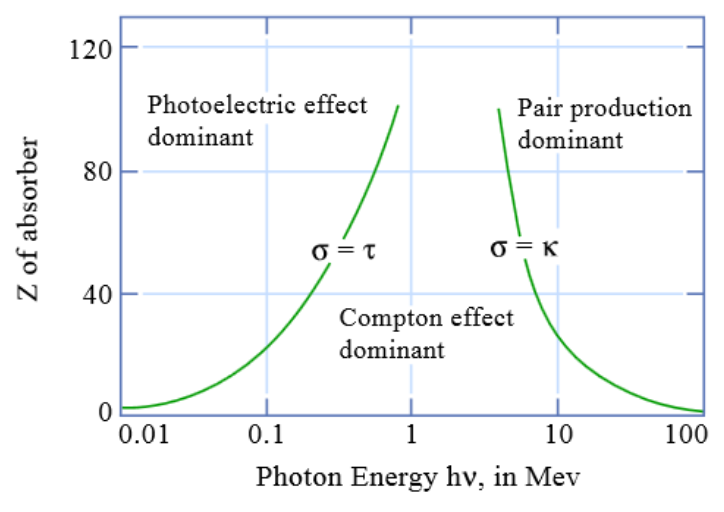
\includegraphics[width=10cm,keepaspectratio]{crosssection.png}
		\caption{Regioni di dominanza delle tre modalità di interazione dei fotoni con la materia, per diverse energie dei fotoni e diverso numero atomico dei bersagli.}
         \label{crosssection}
\end{figure}



\textbf{Terza Esperienza}

\emph{Stimare le quantità di piombo, plastica ($\text{C}_5\text{O}_2\text{H}_8$, $\rho=1,2 g/cm^3$) e paraffina ($\text{C}_{31}\text{H}_{64}$, $\rho=0,9 g/cm^3$) necessarie ad attenuare di un fattore di $10^{-4}$ dei fotoni o fermare elettroni e particelle alfa di energie $0.1$, $1$ e $10$ $MeV$.}

\section{Interazioni Positroni-Materia}

Il positrone prodotto in un decadimento $\beta+$ interagisce in primis per multiple scattering e ionizzazione. Dopodichè esso può fare due cose:

\begin{itemize}
\item Col $20\%$ di probabilità fa annichilazione in volo con un elettrone producendo due fotoni. Ponendoci nel sistema di riferimento dell'elettrone che viene colpito vale la relazione $2m_e+K_e=E_{\gamma1}+E_{\gamma2}$ e l'angolo tra i fotoni è minore di \ang{180}.
\item Con 80\% di probabilità comincia ad orbitare intorno ad un elettrone libero, formando il sistema $e^+e^-$ detto \emph{positronio}.
\end{itemize}

Analizziamo la possibilità della formazione del positronio. Esso a seconda dello spin totale forma l'orto-positronio o il para-positronio. Siccome lo stato di singoletto è uno solo mentre quelli di tripletto sono tre, la formazione di para-positronio (spin totale:$1$)è tre volte più probabile di quella dell'orto-positronio (spin totale:$0$). 
In totale per ogni decadimento che produce un positrone la probabilità di formare para-positronio è 64\%. 
Il para-positronio ha una vita media di $125 ps$ e poi decade in una coppia di fotoni back to back, mentre l'orto-positronio ha una vita media di $140 ns$ e decade in tre fotoni. La coppia di fotoni emessa dal para-positronio è interessante perché se rilevata può dare informazioni per triangolare dove è avvenuto il decadimento. Essi sono emessi a $\ang{180}$ per conservazione della quantità di moto. Inoltre, per conservazione dell'energia, i due fotoni sono esattamente da $511 keV$.
Proprio su questi principi si basa la PET, che per immissione di un radiofarmaco metabolico che decade $\beta+$, triangolando i fotoni, permette di fare diagnostica funzionale.
Il limite principale della PET è il fatto che i positroni prima di formare positronio si muovono nel corpo per scattering multiplo e ionizzazione, variando la loro posizione e dunque creando un incertezza sulla misura finale.
Risoluzione massima: $0,44 mm$.

Approfondimenti e bibliografia: \cite{PET1} \cite{PET2}



% !TEX root = main.tex

\chapter{Decadimenti Nucleari}

I decadimenti nucleari sono tutte quelle reazioni del tipo:

\begin{equation}
X \longrightarrow Y + \sum_C A_C
\end{equation}

In cui c'è il vincolo $m_x>m_y + \sum m_C$

L'uguaglianza esatta è $m_x=m_y+T_y+\sum (m_c+T_c)$, da cui:

\begin{equation}
m_x-m_y-\sum m_c = T_y + \sum T_c = Q_{\text{value}}
\end{equation}

Il $Q_{\text{value}}$ rappresenta la massima energia cinetica assumibile dai prodotti di decadimento nel sistema di riferimento solidale all'atomo instabile. Dal fatto che sia un decadimento consegue che $Q>0$. 


\section{Il Nucleo Atomico}

Per nuclei leggeri la stabilità è verificata quando $Z=N$ ma all'aumentare del numero atomico il numero di neutroni necessario a garantire stabilità aumenta. 
La figura (\ref{curvadistabilita}) rappresenta la curva di stabilità comparata con la retta $Z=N$.\\
\begin{figure}
\centering
		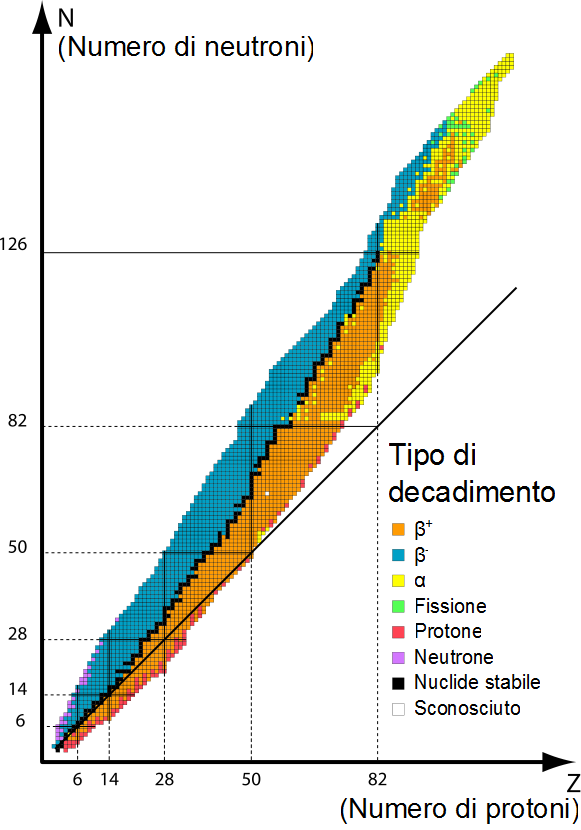
\includegraphics[width=7cm, keepaspectratio]{figs/curvadistabilita.png}
		\caption{Curva di stabilità dei nuclei in funzione del numero di protoni e numero di neutroni. Sono rappresentati anche i decadimenti che tende a fare ogni elemento fuori dalla curva di stabilità.}
         \label{curvadistabilita}
\end{figure}

Due atomi si dicono:

\begin{itemize}
\item Isotopi, se hanno stesso numero atomico;
\item Isotoni, se hanno stesso numero di neutroni;
\item Isobari, se hanno stesso numero di massa.
\end{itemize}

Neutroni e protoni sono fermioni di spin $1/2$. Essi dunque si organizzano nel nucleo su livelli energetici in cui si dispongono a spin opposti.
Quando il numero di neutroni e protoni è pari, ogni livello energetico è riempito. Quando invece il loro numero è dispari, sono più probabili reazioni nucleari al fine di arrivare in livelli energetici più stabili. Ad esempio riempiendo i livelli energetici del $^{12}_5B$ ho un neutrone extra su un livello energetico più alto di quelli riempiti dai protoni. Questo elemento infatti decade $\beta$ nel $^{12}_6C$.
Per differenziare isotopi diversi si usano spettrometri di massa, in cui, sfruttando la forza di Lorenz generata da un campo magnetico, osservo la correlazione tra raggio di curvatura e massa dell'isotopo considerato.
Per misurare invece il raggio nucleare si osserva il pattern di diffrazione dello scattering di elettroni su tale nucleo. Graficando l'intensità dello scattering in funzione dell'angolo, ho la seguente relazione per il primo punto di minimo dell'andamento:

\begin{equation}
\sin \theta^*=0,16\frac{hc}{pcR}
\end{equation}

\begin{figure}
\centering
		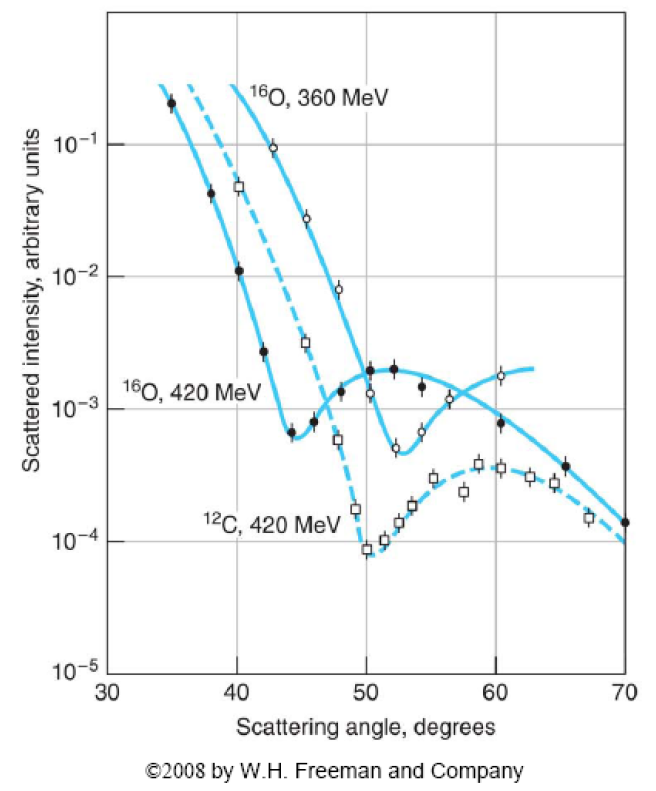
\includegraphics[width=7cm, keepaspectratio]{figs/scatteringatomicradius.png}
		\caption{Andamento dell'angolo di scattering di elettroni su nuclei di ossigeno e carbonio.}
         \label{scatteringatomicradius}
\end{figure}

Da cui si può ricavare il raggio.

Empiricamente abbiamo la seguente legge che lega raggio nucleare e massa atomica:

\begin{equation}
R=1,15A^{1/3} (fm)
\end{equation}

Guardando la tavola periodica in Figura (\ref{atomicradii}) si può dire che gli elementi presenti in natura più grandi sono quelli in basso a sinistra più i gas nobili.
Consideriamo ora la densità nucleare. 

\begin{figure}
\centering
		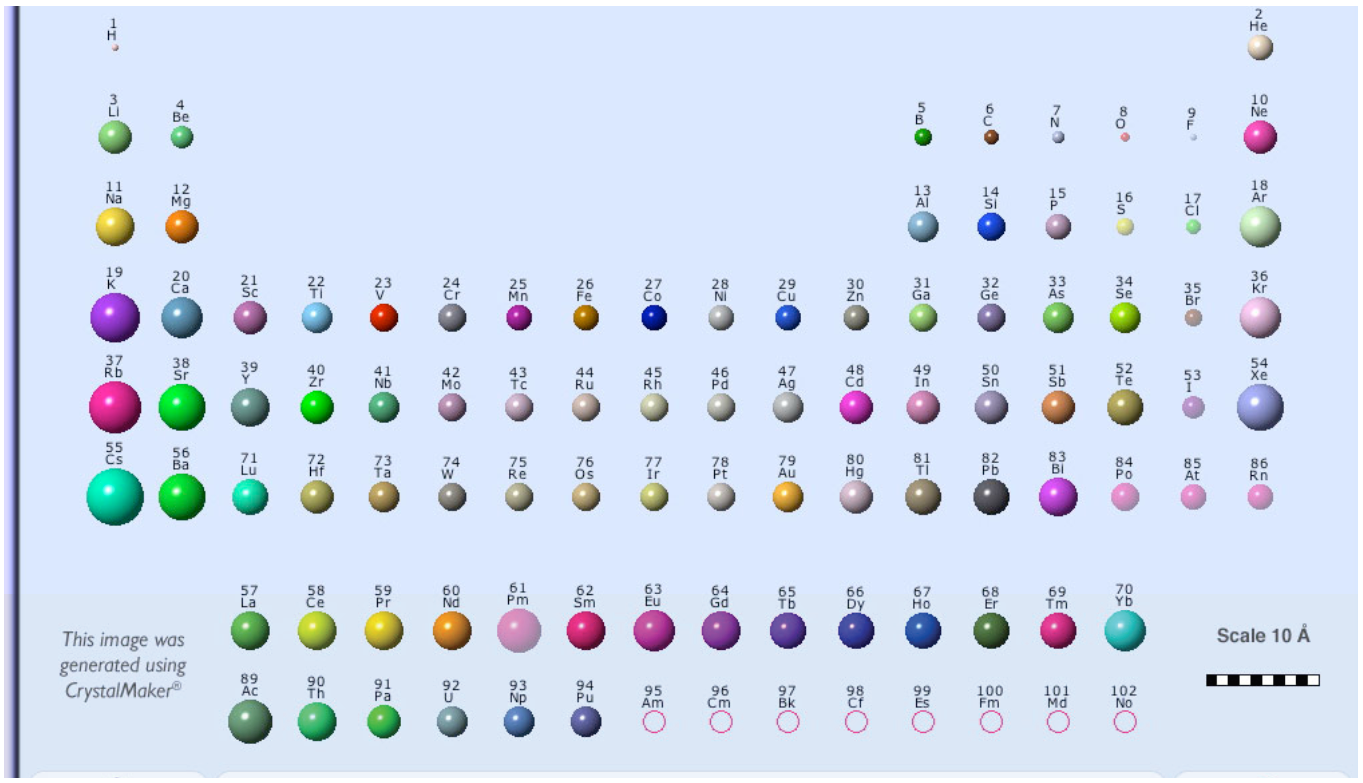
\includegraphics[width=16cm, keepaspectratio]{figs/atomicradii.png}
		\caption{Tavola periodica. Sono evidenziati i raggi di ogni elemento.}
         \label{atomicradii}
\end{figure}

\begin{equation}
\rho=\frac{m}{\frac{4}{3}\pi R^3}=\frac{Am_p}{\frac{4}{3}\pi (1,15 A^{1/3})^3}=\frac{m_p}{\frac{4}{3}\pi 1,15^3 (fm^3)} = 10^{17} kg/m^3
\end{equation}

Ovvero essa è in prima approssimazione indipendente dal tipo di atomo. 
Altra verifica che questa sia la densità del nucleo atomico è che essa risulta essere la densità delle nane bianche, stelle in cui i nucleoni sono compressi uno contro l'altro.
                                                                                                                    
Per ricavare con maggiore precisione la massa atomica smettiamo di trascurare la differenza in massa tra neutroni e protoni e consideriamo anche l'energia di legame tra i nucleoni nel nucleo. Abbiamo allora che:

\begin{equation}
M(Z,A)=Z\times m_p+(A-Z)\times m_n-A\times BindingEnergy
\end{equation}

\textbf{Quarta Esperienza}

\begin{itemize}
\item \emph{Graficare la massa nucleare in funzione di Z per $A=18$ e $A=208$. Comparare il risultato con il grafico dei tempi di decadimento.}
\item \emph{Graficare Sp(Z) e Sn(Z) per $N=9$.}
\item \emph{Graficare Sp(N) e Sn(N) per $Z=33$.}
\end{itemize}


\section{Grandezze Importanti}

Quando un nucleo è instabile ha una certa probabilità per unità di tempo di decadere in un nucleo stabile, detta \emph{costante radioattiva} $\lambda$. 
Indicando con $N$ il numero di nuclei instabili, il numero medio di nuclei che decadono nell'unità di tempo è dato da $\lambda N$. Questa grandezza complessiva è detta \emph{attività}. Nel tempo tra $t$ e $t+dt$ il numero di nuclei varia al seguente modo:

\begin{equation}
\mathrm{d}N=-\lambda N \mathrm{d}t
\end{equation}

Risolvendo l'equazione differenziale si ottiene

\begin{equation}
N(t)=N(0)e^{-\lambda t}
\end{equation}

Osserviamo che il cosiddetto tempo di dimezzamento, ovvero il tempo al quale il numero di nuclei attivi è dimezzato, è dato da

\begin{equation}
\tau_{\frac{1}{2}}=\frac{\ln2}{\lambda}
\end{equation}

Ricordando che l'attività è definita come $\lambda N$, moltiplicando l'equazione precedente per $\lambda$ ottengo l'andamento temporale dell'attività:

\begin{equation}
A(t)=\lambda N(t)=A(0)e^{-\lambda t}
\end{equation}

L'unità di misura dell'attività era stata per convenzione stabilita essere il Curie, corrispondente a 37 miliardi di disintegrazioni al secondo, indicata con $\text{Ci}$. Essa è approssimativamente l'attività di un grammo di $^{226}\text{Ra}$.
Attualmente l'unità di misura più usata è diventata una disintegrazione al secondo, detta Bequerel, indicata $\text{Bq}$.
In laboratorio si usano di solito sorgenti dell'ordine del $\text{kBq}$. Dalle definizioni delle unità di misura segue il cambio:

\begin{equation}
1 \text{Ci} = 3,7 \times 10^{10} \text{Bq}
\end{equation}

Un atomo può decadere in canali diversi, ognuno con la sua vita media (e dunque la sua costante radioattiva). Allora si definisce la costante radioattiva totale $\lambda_{tot}=\sum \lambda_{i}$. Si introduce la branching fraction come $\text{BR}=\frac{\lambda_i}{\lambda_{tot}}$.

\emph{Nota: l'attività non tiene conto del tipo di fenomeno che sta avvenendo e di quante particelle genera. è un conto di quanti decadimenti avvengono, qualsiasi essi siano e qualunque numero di particelle producano. Per contare nello specifico il numero di un certo tipo di decadimento che avviene si usano gli Hz o i CPS (Counts Per Second)}

Si definiscono le seguenti grandezze importanti:
\begin{itemize}
\item Attività Specifica: $A_{sp}=\frac{\mathrm{d}A}{\mathrm{d}V}$
\item Standard Uptake Value (SUV): $\text{SUV}=\frac{A_{sp}(\text{tumore})}{A(\text{somministrata})}$ per renderla adimensionale si fa $\text{SUV}=\frac{A_{sp}(\text{tumore})}{A(\text{somministrata})\times \rho}m_{\text{paziente}}$
\item Tumor Non-tumor Ratio (TNR): $\text{TNR}=\frac{\text{SUV}(\text{tumore})}{\text{SUV}(\text{limitrofo})}$
\end{itemize}

In genere si cerca $\text{SUV}\sim5$

\section{Decadimenti alpha}

Si definiscono decadimenti $\alpha$ quelli della seguente forma:

\begin{equation}
^A_Z X \longrightarrow ^{A-4}_{Z-2}Y + ^4_2He
\end{equation}

Siccome i prodotti di reazione sono due, nel sistema di riferimento dell'atomo che decade essi sono prodotti back to back con stesso impulso per conservazione della quantità di moto. Allora valgono le seguenti uguaglianze:

\begin{equation}
Q=T_y+T_{\alpha}=\frac{p^2}{2m_y}+\frac{p^2}{2m_{\alpha}}=\frac{m_{\alpha}}{m_y}T_{\alpha}+T_{\alpha}
\end{equation}

Da cui

\begin{equation}
T_{\alpha}=\frac{Q}{1+\frac{m_{\alpha}}{m_y}} 
\end{equation}

Da cui si deduce che per decadimenti di atomi molto massivi, in cui anche $Y$ è molto massivo, ho $T_{\alpha}\simeq Q$.

\emph{Nota: un decadimento può portare alla creazione di un prodotto che non è nel suo stato di spin nucleare fondamentale, ma ci decade emettendo raggi $\gamma$ }

Si osserva che c'è una relazione tra la vita media di un certo radionuclide e l'energia con cui vengono emesse le particelle $\alpha$: è la legge di Geiger-Nuttall:

\begin{equation}
\log \tau = a + b \log (E)
\end{equation}

\emph{Nota: si usa il $^{223}Ra$ per curare le metastasi nelle ossa o nella prostata perché mima il Calcio}

\section{Fissione Spontanea}

La fissione spontanea consiste nel decadimento di un nucleo pesante in due nuclei più leggeri con probabile produzione di neutroni. Esso è un processo altamente improbabile perché la barriera di potenziale da superare per farla avvenire è altissima. Il nucleo più leggero per cui si osserva è $^{226}Ra$, mentre quelli per cui la probabilità di fissione è paragonabile a quella di decadimento $\alpha$ sono alcuni isotopi dell'uranio. La fissione spontanea diventa dominante tra i branching ratio solo per $A>260$.
I prodotti di fissione sono normalmente lontani dalla curva di stabilità e decadono $\beta-$. 
Essi inoltre sono tra loro molto probabilmente asimmetrici: il valore più probabile di differenza di numero di massa tra i prodotti di fissione è circa $45$.

\begin{figure}
\centering
		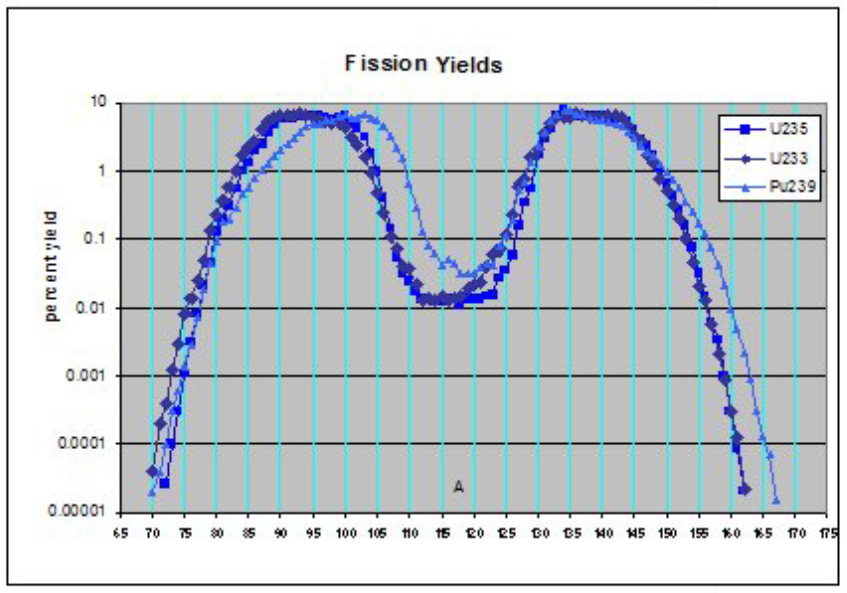
\includegraphics[width=12cm, keepaspectratio]{figs/fissionyealds.png}
		\caption{Distribuzione di probabilità dei prodotti della fissione dell'$^{235}\text{U}$, del $^{233}\text{U}$ e del $^{239}\text{Pu}$. Si osserva che la produzione di due nuclei con massa simile è improbabile. Molto più probabile è la produzione di un nucleo pesante ed un nucleo leggero.}
         \label{fissionyealds}
\end{figure}

\section{Decadimenti Beta}

I decadimenti beta sono trasformazioni isobariche che avvengono per interazione debole e includono la presenza di un elettrone o un positrone. Sono di tre tipi:

\begin{equation}
\beta-: \qquad n \longrightarrow p + e^-+\bar{\nu_e}  \quad ovvero, atomicamente \quad  ^A_ZX \longrightarrow _{Z+1}^AY+e^-+\bar{\nu_e}
\end{equation}


\begin{equation}
\beta+: \qquad p \longrightarrow n + e^++\nu_e \quad ovvero, atomicamente \quad  ^A_ZX \longrightarrow _{Z-1}^AY+e^++\nu_e
\end{equation}


\begin{equation}
CE: \qquad p + e^- \longrightarrow n + \nu_e \quad ovvero, atomicamente \quad  ^A_ZX+e^- \longrightarrow _{Z-1}^AY+\nu_e
\end{equation}

Osserviamo che tutte sono reazioni che conservano il numero di massa totale dell'atomo ma cambiano il suo numero atomico.
Fuori dal nucleo è impossibile che avvengano decadimenti $\beta+$ perché la massa del protone è inferiore a quella del neutrone. Invece le reazioni $\beta-$ avvengono velocissime fuori dal nucleo, ed è per questo che non esistono neutroni liberi.
Osserviamo inoltre che quando avviene cattura elettronica tutti gli altri elettroni devono riaggiustarsi scendendo ai livelli inferiori, emettendo intensa radiazione X.
Per i decadimenti $\alpha$ avevamo visto che siccome c'era un prodotto massivo e l'$\alpha$ leggera allora il Q value andava tutto all'energia cinetica della particella $\alpha$. In questo caso invece sono due i prodotti leggeri: neutrino ed elettrone o positrone.

 Come si può vedere nelle figure (\ref{qbetapiu}) e (\ref{qbetameno}) le distribuzioni di energia con cui vengono prodotti elettroni e positroni sono diverse perché è diverso il loro Q value. Nelle seguenti equazioni le maiuscole sono le masse atomiche, minuscole le masse nucleari (la differenza è la massa degli elettroni).

\begin{figure}
\centering
		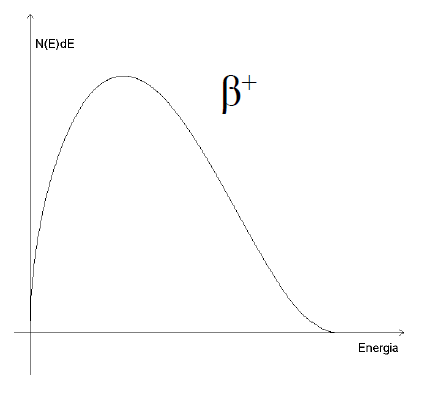
\includegraphics[width=5cm, keepaspectratio]{figs/qbetapiu.png}
		\caption{Distribuzione dell'energia del positrone prodotto in un decadimento $\beta+$. La probabilità che esso abbia energia nulla è zero, perché}
         \label{qbetapiu}
\end{figure}

\begin{figure}
\centering
		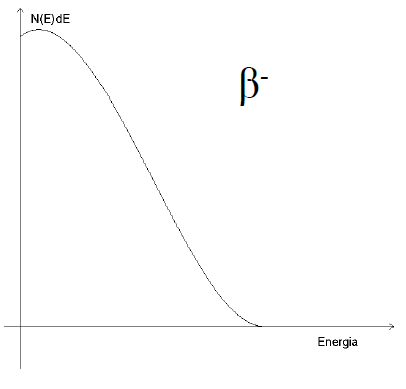
\includegraphics[width=5cm, keepaspectratio]{figs/qbetameno.png}
		\caption{Distribuzione dell'energia dell'elettrone prodotto in un decadimento $\beta-$.}
         \label{qbetameno}
\end{figure}

\begin{equation}
M_x=m_x+Zm_e 	\qquad M_y=m_y+(Z+1)m_e
\end{equation}

\begin{equation}
Q_{\beta^-}=m_x-m_y-m_e
\end{equation}

è facile osservare che $M_x-M_y=m_x-m_y-m_e$. Allora possiamo dire:

\begin{equation}
Q_{\beta^-}=M_x-M_y
\end{equation}

Ciò ci dice anche che condizione necessaria e sufficiente a far avvenire un decadimento $\beta^-$ è che la massa del nucleo padre sia maggiore della massa del nucleo figlio.

Per il decadimento $\beta^+$ invece:

\begin{equation}
M_x=m_x+Zm_e \qquad M_y=m_y+(Z-1)m_e
\end{equation}

\begin{equation}
Q_{\beta^+}=m_x-m_y-m_e
\end{equation}

Si osserva facilmente che $M_x-M_y=m_x-m_y+m_e=Q_{\beta^+}+2m_e$.
Ovvero

\begin{equation}
Q_{\beta^+}=M_x-M_y-2m_e
\end{equation}

Allora condizione necessaria e sufficiente a far avvenire un decadimento $\beta^+$ è che la differenza di masse atomiche tra nucleo padre e nucleo figlio sia almeno due volte la massa dell'elettrone: $M_x-M_y>2m_e$.

In natura, con l'eccezione del $^{40}K$, non esistono radionuclidi che decadono $\beta^+$, vengono prodotti artificialmente.

Il punto estremo della distribuzione di energie degli elettroni in queste due reazioni è detto End Point, ed è dato da quegli elettroni che estraggono tutta l'energia dal Q value.

Un nucleo può \emph{catturare un elettrone} dalla shell atomica, trasformare un protone in neutrone ed emettere un neutrino con la seguente reazione:

\begin{equation}
^A_ZX+e^- \longrightarrow _{Z-1}^AY+\nu_e
\end{equation}

Data la pesantezza di $Y$ rispetto al neutrino, quest'ultimo viene praticamente emesso sempre con la stessa energia. In questo caso il Q value ci pone il seguente vincolo:

\begin{equation}
M_x+m_e>M_y
\end{equation}

Allora riassumendo in scala di energie crescente i decadimenti possibili sono i seguenti:

\begin{itemize}
\item Cattura Elettronica se $M_x-M_y>-m_e$
\item Decadimento $\beta^-$ se $M_x-M_y>0$
\item Decadimento $\beta^+$ se $M_x-M_y>2m_e$
\item Decadimento $\alpha$ se $M_x-M_y>m_{\alpha}$
\end{itemize}

\textbf{Quinta Esperienza}

\begin{itemize}
\item \emph{Trovare una lista di isotopi di C, Na, F, P, Ga, I, Re, Lu, Y e Sr con decadimenti $\beta+$ e $\beta-$ dominanti con un tempo di dimezzamento compreso tra 1 minuto e 10 giorni.}
\item \emph{Per ogni isotopo scrivere tempo di dimezzamento, end point e range proiettato per energie che siano pari a metà dell'end-point.}
\end{itemize}



Un applicazione del decadimento $\beta^-$ è la Brachioterapia \cite{Brachioterapia}, che consiste nello spalmare pomate emettenti elettroni sui tumori. Il LET degli elettroni abbiamo visto che è molto corto e concentrato all'inizio grazie al multiple scattering. Si cercano elementi ad alto End Point. Gli elementi più usati sono:
\begin{itemize}
\item $^{90}\text{Y}$ per il fegato,
\item $^{188}\text{Re}$ per la pelle,
\item $^{32}\text{P}$ per il cervello,
\item $^{90}\text{Sr}$ per fegato e polmoni.
\end{itemize}

Ognuno di questi ha endpoint dell'ordine del MeV e range proiettato dell'ordine del millimetro.
Si usa inoltre per la terapia radiometabolica, in cui i radionuclidi sono attaccati a molecole che vengono metabolizzate dai tumori. Gli elementi più usati sono:

\begin{itemize}
\item $^{90}\text{Y}$ per i tumori neuroendocrini,
\item $^{131}\text{I}$ $^{132}\text{I}$ per la tiroide,
\item $^{177}\text{Lu}$ per i tumori neuroendocrini.
\end{itemize}

La tipica iniezione è di $3 \text{MBq/kg}$

Altra applicazione è la \emph{Chirurgia Radioguidata} in cui si inserisce un tracciatore che decade $\beta^-$, tipo $^{90}\text{Y}$, e un detector di elettroni da passare sul punto da operare. Lo svantaggio è che bisogna sviluppare un tracciatore specifico per ogni caso. Quì è stato inventato PROBE.

Ancora un'altra applicazione: la PET usa decadimenti $\beta^+$ insieme a radiofarmaci funzionali per fare uno scan delle coppie gamma prodotte dal positronio. In questo caso voglio basso End Point. Gli elementi più usati sono:

\begin{itemize}
\item $^{18}\text{F}$ generico,
\item $^{11}\text{C}$ per prostata e cervello,
\item $^{68}\text{Ga}$ per tumori neuroendocrini,
\item $^{13}\text{N}$ per la pelle.
\end{itemize}

Infine osservando i prodotti di reazione posso fare una valutazione della Dose che ha attraversato il paziente.

\section{Emissione gamma}

I nuclei risultanti da decadimenti $\beta$ possono trovarsi in stati diversi da quello fondamentale. In tal caso esso cadrà negli stati più bassi in energia emettendo raggi $\gamma$. La transizione può avvenire con un unico salto e produzione di un fotone molto energetico, o con più salti intermedi e la produzione di una cascata di raggi $\gamma$. Si dice emissione gamma e non decadimento gamma perché non c'è correlazione tra il numero di atomi che scende allo stato fondamentale e il numero di fotoni emessi. La vita media di tali stati è dell'ordine del picosecondo, poco più di quella dei decadimenti beta. Ci sono alcune eccezioni, date da stati metastabili, tipo il $^{99m}\text{Tc}$ metastabile prodotto dal decadimento beta- del $^{99}\text{Mo}$ per cui la vita media è 6 ore.
L'emissione gamma è in competizione con un altro fenomeno che può avvenire con un nucleo in stato eccitato: la \emph{Conversione Interna}. Ciò consiste nel fenomeno per cui l'energia in eccesso del nucleo viene direttamente trasferita ad un elettrone che viene ionizzato ed assume energia finale:

\begin{equation}
E_{e^-}=E_{s.eccitato}-I
\end{equation}

\emph{Nota: Per possibili decadimenti gamma con le loro probabilità si consulta questo sito: \href{http://nucleardata.nuclear.lu.se/toi/nucSearch.asp }}

Un'applicazione di questo fenomeno è la SPECT (Single Photon Emission Computed Tomography). Ogni decadimento porta all'emissione di un fotone. Si mette in circolazione una sostanza radioattiva che va nell'organo di interesse ed emette un fotone. Il rilevatore mi dice energia e direzione del fotone usando varie fessure che selezionano la direzione. Voglio un cammino libero di 10cm così che riesca ad uscire dal corpo del paziente. Il rilevatore deve essere un calorimetro molto assorbente e con setti molto lunghi e densi. L'elemento che cerco è il $^{99m}\text{Tc}$.

Altra applicazione è la Teragnostica: si fa con elementi che decadono sia $\beta-$ che $\gamma$ così da fare terapia e diagnostica rispettivamente. Elementi utili a ciò sono $^{177}\text{Lu}$ e $^{131}\text{I}$.

Ai fini di monitorare la dose come visto prima si possono usare gli elettroni dei decadimenti beta ma ci mettono troppo ad uscire. Invece i raggi $\gamma$ prodotti nella reazione danno informazioni immediate su dove si sta rilasciando la dose.

Ultima applicazione è la radioterapia con il cobalto. Il $^{60}\text{Co}$ decade $\beta-$ e i suoi prodotti decadono $\gamma$. Allora il paziente riceve un elettrone e due fotoni. I pazienti inoltre vedono live la loro risonanza magnetica e possono aggiustarsi per rimanere nella zona di interesse. La dose è monitorata live quindi se il paziente si muove e fa uscire il target dalla zona di interesse il fascio si spegne.

\section{Equilibrio Secolare}

Un fenomeno interessante si verifica quando un nucleo padre con tempo di vita medio $\tau_f$ decade in un nucleo figlia con tempo di vita $\tau_d$ una frazione $\Phi$ di volte. Ricordando che abbiamo definito l'attività come $A=\lambda N=\frac{N(0)}{\tau}e^{-t/\tau}$, segue che, guardando il numero totale di nuclei figlie che ho, esso aumenta per produzione dal padre e diminuisce per decadimento:

\begin{equation}
\frac{dN_d}{dt}=-\Phi \frac{dN_f}{dt} - \frac{\partial N_d}{\partial t} = \Phi \frac{N_f}{\tau_f} - \frac{N_d}{\tau_d}
\end{equation}

Integrando ottengo

\begin{equation}
N_d(t)=\frac{\Phi}{\frac{\tau_f}{\tau_d}-1}N_f(0)(e^{-t/\tau_f}-e^{-t/\tau_d})
\end{equation}

Per finire rendiamola un'attività dividendo per $\tau_d$, ma esprimiamo $A_f(0)$ al posto di $N_f(0)$. Otteniamo:

\begin{equation}
A_d(t)=\frac{\Phi}{\frac{\tau_f}{\tau_d}-1}A_f(0)\frac{\tau_f}{\tau_d}(e^{-t/\tau_f}-e^{-t/\tau_d}) =\frac{\Phi}{1-\frac{\tau_d}{\tau_f}}A_f(0)(e^{-t/\tau_f}-e^{-t/\tau_d})
\end{equation}

Analizziamo adesso i casi limite. Se $\tau_d << t << \tau_f$, come nel $^{99}\text{Mo} \rightarrow ^{99m}\text{Tc}$, avrò:

\begin{equation}
A_d(t)=\Phi A_f(t)
\end{equation}

Ovvero l'attività del nucleo figlia sarà solo scalata di un certo fattore rispetto a quella del padre.

Invece quando ho $\tau_f \sim t << \tau_d$ , come nel $^{223}\text{Ra}$, ottengo:

\begin{equation}
A_d(t)=\Phi \frac{\tau_f}{\tau_d}A_f(0)(\-e^{-t/\tau_f})
\end{equation}

Torniamo al primo caso e osserviamo cosa succede se estraiamo i nuclei figlie dopo una vita media $\tau_d$. Grafico.

Si possono creare dei generatori continui di Tecnezio con macchinari contenenti Molibdato $^{99}\text{MoO}_4^{2-}$ e Pertecnato $^{99m}\text{TcO}_4^-$.
Altri esempi sono le famiglie naturali dell'$^{238}\text{U}$, $^{232}\text{Th}$ e $^{235}\text{U}$.  Le attività di una famiglia sono tutte legate tra loro dalle equazioni differenziali di Bateman.

Osserviamo un esempio: $^{90}\text{Sr} \rightarrow ^{90}\text{Y} \rightarrow ^{90}\text{Zr}$. Quando prendo una certa quantità di Becquerel di $^{90}\text{Sr}$ sto prendendo anche la stessa attività di ittrio a meno di un fattore $\Phi$. Qui si vede la differenza tra rate e attività: prendendo $1 \ Bq$ di stronzio ho $2 \ kHz$ di produzione di elettroni, uno dal decadimento dello Stronzio e uno dal decadimento dell'Ittrio. 

\textbf{Sesta Esperienza}

\emph{Trovare coppie di nuclei padre-figlia in cui:}
\begin{itemize}
\item \emph{La figlia decade $\beta$ con $\tau\sim1-100\text{hr}$}
\item \emph{Il padre decade con $\tau\sim100\text{d}-10\text{y}$}
\end{itemize}



% !TEX root = main.tex

\chapter{Reazioni Nucleari}

Per le reazioni nucleari c'è una specifica nomenclatura. Esponiamola con un esempio. La seguente reazione:

\begin{equation}
\alpha+^{14}_7N \longrightarrow p+^{17}_8O
\end{equation}

Viene indicata con $^{14}N(\alpha,p)^{17}O$. In generale si indica:

\begin{equation}
\text{Nucleo}_i(\text{proiettile},\text{frammento})\text{Nucleo}_f
\end{equation}

Le reazioni nucleari possono essere categorizzate come segue:

\begin{itemize}
\item Fotodisintegrazione Nucleare: un fotone inizializza una reazione: $X(\gamma,*)Y$
\item Cattura Neutronica o Protonica Radioattiva: un nucleo cattura un nucleone emettendo $\gamma$: $X(n/p,\gamma)Y$
\item Scattering Elastico: canali d'entrata e uscita identici, nessuno stato eccitato: $X(a,a)X$
\item Scattering Inelastico: nel canale d'uscita uno o più prodotti sono in stati eccitati: $X(a,a)X^* \rightarrow X(a,a+\gamma)X$
\end{itemize}

Per i decadimenti nucleari avevamo che il Q-value doveva sempre essere maggiore di 0. Nelle reazioni esso può assumere segno diverso, portando a tre tipi di reazioni:

\begin{itemize}
\item $Q>0$: reazioni esotermiche, ovvero spontanee, tipo fissione, fusione. Nessuna condizione sull'energia cinetica del proiettile.
\item $Q=0$: reazioni elastiche.
\item $Q<0$: reazioni endotermiche, ovvero per avvenire l'energia cinetica del proiettile deve essere sopra una certa soglia.
\end{itemize}

Nel sistema della particella b, l'energia cinetica di soglia risulta essere

\begin{equation}
T_a>\frac{(\sum m_c)^2-(m_a+m_b)^2}{2m_b}
\end{equation}

Dove bisogna stare attenti all'espressione delle masse dei nuclei: siccome il numero di protoni e neutroni si conserva nelle reazioni nucleari, è importante tenere conto delle binding energy nel conto complessivo. \\
Nei prossimi paragrafi approfondiremo alcuni tipi di reazioni nucleari specialmente interessanti per le loro applicazioni 

\section{Produzione di Radioisotopi}

Alcune sostanze stabili possono essere rese radioattive sottoponendole a bombardamento di neutroni o protoni. Il modello matematico che descrive l'andamento dell'attività della sostanza così prodotta è molto simile a quello di nuclei padri e figlie visto nel capitolo sui decadimenti nucleari. 
Immaginiamo di avere un flusso $\Phi_p$ di protoni incidenti su un nucleo inizialmente stabile con sezione d'urto per l'attivazione $\sigma_{att}$. Allora il rate con cui avviene l'attivazione sarà

\begin{equation}
P=\Phi_p \sigma_{att} n_Y
\end{equation}

Allora se $\tau_Y$ è la vita media dell'Y attivato, l'andamento del numero di nuclei Y sarà:

\begin{equation}
\frac{\mathrm{d}N_Y}{\mathrm{d}t}=-\frac{N_Y}{\tau_Y}+P
\end{equation}

Integrando si ottiene

\begin{equation}
N_Y(t)=P\tau_Y(1-e^{-t/\tau_Y})
\end{equation}

Da cui si vede che nel tempo l'attività raggiunge un asintoto dato da $A=P$, che in tale asintoto $\frac{\mathrm{d}N_Y}{\mathrm{d}t}=0$ e che sempre in tale asintoto $P=\frac{N_Y}{\tau_Y}$.

Osservando l'andamento vicino all'origine, per tempi molto brevi, sviluppando al primo ordine l'andamento dell'attività, ottengo:

\begin{equation}
A(\Delta t)=\frac{P \Delta t}{\tau_Y}
\end{equation}

Ovvero aumenta in maniera lineare. Rimuovendo un quantitativo di radioisotopo posso osservare il suo andamento e ricavare la rate di produzione iniziale P.

\section{Frammentazione}

Se il proiettile nella reazione nucleare è massivo, può frammentarsi. La reazione generica ha la forma seguente:

\begin{equation}
x+X \longrightarrow a+b+X
\end{equation}

In una reazione del genere avremo i seguenti vincoli:

\begin{itemize}
\item $m_a, m_b  \ < \ m_x$ perché risultati di una frammentazione. L'uguaglianza non vale perché si è persa della massa che era binding energy nucleare.
\item $Z_a, Z_b \ < \ Z_x$ perché la somma dei protoni dei due prodotti di frammentazione deve essere il numero di protoni del proiettile.
\item $\beta_a, \beta_b \ >> \ \beta_x$ perché sono meno massivi e c'è il rilascio di energia della binding energy.
\end{itemize}

Essendo i prodotti di reazione più veloci e meno carichi, la loro perdita di energia nell'unità di percorso è minore e dunque il loro range è molto maggiore di quello del proiettile originale. 
In altre parole i prodotti di frammentazione penetrano di più del proiettile.
Nella radioterapia a energie maggiori e proiettili più pesanti corrispondeva un LET più piccato intorno al range, ma da questo fenomeno risulta che se tali energie fossero troppo alte, e tali proiettili troppo pesanti, potrebbero risultare in prodotti di frammentazione energetici e più penetranti che danneggerebbero il paziente. Questo è il motivo per cui nell'adronterapia non si usano nuclei più pesanti del carbonio.

\section{Attivazione Neutronica}
\`E un fenomeno che si sfrutta nella \emph{Neutron Activation Analysis} nello studio della composizione di un certo materiale. Consiste nell'acquisizione di un neutrone libero da parte di un nucleo in deficienza di neutroni. A questa acquisizione segue l'emissione di un fotone $\gamma$ con una specifica energia:

\begin{equation}
E_{\gamma}=E_{Y^*}-E_{Y}
\end{equation}



% !TEX root = main.tex

\chapter{Dosimetria}
La dosimetria è una branca a cavallo tra la fisica e la medicina che definisce le grandezze fisiche che hanno la maggior probabilità di essere correlate a grandezze cliniche (quale la sopravvivenza dei pazienti). Questa quantificazione e' necessaria sia per esposizioni accidentali alla radiazioni, quali nel caso di incidenti nucleari, che per esposizioni intenzionali a radiazioni per fini terapeutici. Partiamo considerando alcuni ordini di grandezza:
Vi sono circa $10^{13}$ cellule nel corpo umano, ognuna con un diametro medio di $10 \ \mu m$, con un nucleo di $3 \ \mu m$ contenente DNA, che ha una larghezza tipica di $ 2 \ nm$ e la lunghezza di un gene è circa $0,1 \ \mu m$. 

Esistono due modi in cui una radiazione incidente può provocare la morte di una cellula, uno diretto ed uno indiretto. Per uccidere direttamente una cellula la radiazione incidente deve rompere legami in entrambe le eliche di un tratto del suo DNA in modo da renderlo difficilmente reparabile, perché nessuna delle due eliche potrà fare da stampo per la rigenerazione dell'elica complementare. \\
Ciò che accade più frequentemente però è che la cellula venga uccisa dalla radiazione incidente in modo indiretto. Questo avviene quando la radiazione ionizza le molecole d'acqua presenti nella cellula creando specie reattive come $\text{OH}^{-}$, $\text{O}_2^{-}$ e $\text{H}_2\text{O}_2$ che possono attaccare direttamente il DNA o portare alla sintetizzazione di altre sostanze analoghe a quelle adoperate nella chemioterapia che uccidono la cellula o ne inibiscono la riproduzione.\\
Gli effetti della radiazione possono essere distinti in stocastici o non-stocastici. Gli effetti stocastici sono quelli che sono privi di un livello di soglia di esposizione sotto il quale non vi sono effetti: ad ogni livello di esposizione dalla radiazione corrisponde una probabilità che si verifichino tali effetti, e la loro gravità non dipende dall'intensità della radiazione. Gli effetti non stocastici invece sono prevedibili ed avvengono oltre un certo livello di intensità di radiazione. La loro gravità inoltre dipende dall'intensità della radiazione.\\
Infine i danni da radiazione si possono dividere in somatici e genetici, a dipesa dal fatto che le cellule colpite siano quelle somatiche o quelle germinali.


\section{Grandezze Preliminari}

Si definiscono le seguenti grandezze:

\begin{itemize}
\item Fluenza $\phi=\frac{\mathrm{d}N}{\mathrm{d}A}$ è una proprietà strettamente della sorgente, come l'attività.
\item Flusso $\Phi=\frac{\mathrm{d}N}{\mathrm{d}A\mathrm{d}t}$
\item Fluenza di Energia $\psi=\frac{\mathrm{d}E}{\mathrm{d}A}$
\item Flusso di Energia $\Psi=\frac{\mathrm{d}E}{\mathrm{d}A\mathrm{d}t}$
\end{itemize}

\section{Esposizione}

L'esposizione, o exposure, è una grandezza esclusivamente legata alla radiazione neutra. \'E definita nel seguente modo:

\begin{equation}
X=\frac{\mathrm{d}q}{\mathrm{d}m}=\frac{1}{\rho}\frac{\mathrm{d}q}{\mathrm{d}V}
\end{equation}

Essa rappresenta la quantità di carica del mezzo che viene accelerata quando esso è investito da radiazione, per unità di massa. La sua unità di misura è la seguente:

\begin{equation}
1 Roentgen = 2,58 \times 10^{-4} \frac{C}{kg}
\end{equation}

C'è un modo indiretto di calcolarla. Se esprimo $\mathrm{d}q=\frac{eE_{\gamma}\mathrm{d}N }{w}$ dove $e$ è la carica dell'elettrone, $E_{\gamma}$ l'energia della radiazione neutra incidente, $\mathrm{d}N$ il numero di cariche accelerate e $w$ è l'energia di ionizzazione media (34 eV in aria), e se esprimo l'unità di massa come $\mathrm{d}m=\rho A \mathrm{d}x$, allora ho:

\begin{equation}
X=\frac{1}{\rho}\frac{e}{w}\frac{E_{\gamma}\mathrm{d}N}{A  \mathrm{d}x}=\frac{e  \mu  N E_{\gamma} }{ w  \rho A}=\frac{e \mu E_{\gamma} \phi}{w \rho}
\end{equation}

Dove si è tenuto conto del fatto che $\frac{N}{A}=\phi$ e che $\frac{\mathrm{d}N}{\mathrm{d}x}=\mu N$.

Spesso si parla di exposure rate, derivata nel tempo dell'exposure.

Nel caso specifico di sorgenti puntiformi di raggi $\gamma$ vale anche la seguente legge:

\begin{equation}
\frac{\mathrm{d}X}{\mathrm{d}t}=\Gamma\cdot\frac{A}{d^2}
\end{equation}

Dove $\Gamma$ è un coefficiente specifico di ogni sorgente, $A$ è l'attività di quella sorgente, $d$ è la distanza da tale sorgente.

\section{Dose}

La dose è definita come l'energia assorbita per radiazione dall'unità di massa del paziente:

\begin{equation}
D=\frac{\mathrm{d}E}{\mathrm{d}m}
\end{equation}

Essa è una proprietà collettiva dell'intero trattamento.

L'energia assorbita può essere esplicitata come segue

\begin{equation}
E=E_{rad_{i}}-E_{rad_{f}}+\sum \text{Q}
\end{equation}

Dove Q è il Q-value delle reazioni che avvengono nel caso considerato, che dunque può avere segno alterno in base al tipo di reazioni. Nel caso di irraggiamento da parte di un flusso di fotoni monocromatico vale la seguente uguaglianza:

\begin{equation}
\mathrm{d}E_{\gamma}=E_{\gamma}\mathrm{d}N
\end{equation}

Dunque la dose può essere espressa come segue:

\begin{equation}
D_{\gamma}=\frac{E_{\gamma}\mathrm{d}N}{\rho A\mathrm{d}x}=\frac{E_{\gamma}\mu N}{\rho A}=\frac{E_{\gamma}\mu \Phi}{\rho} 
\end{equation}

Dove si è tenuto in considerazione il fatto che $\mathrm{d}N/\mathrm{d}x=\mu N$ in modulo.

\textbf{E nel caso di un flusso di fotoni non monocromatico?}

Nel caso di irraggiamento da parte di un fascio di particelle cariche invece vale $\mathrm{d}E=N\mathrm{d}E$, dunque la dose viene espressa come segue:

\begin{equation}
D=\frac{N\mathrm{d}E}{\rho \mathrm{d}V}=\frac{N\mathrm{d}E}{\rho A \mathrm{d}x}=\frac{LET\cdot\phi}{\rho}
\end{equation}

In ogni caso l'unità di misura convenzionale è il Gray.

\begin{equation}
1 Gy = 1 \frac{J}{kg}
\end{equation}

\section{Confronto Tra Dose ed Esposizione}

Confrontando l'espressione della dose per i fotoni e l'esposizione, osserviamo che:

\begin{equation}
X=\frac{e}{w}\frac{\mu}{\rho}E_{\gamma}\phi=\frac{e}{w}D
\end{equation}

Ora, sapendo che $\frac{w_{aria}}{e}=8,74\cdot 10^{-3} \ Gy/R$ possiamo calcolare la dose in qualunque materiale conoscendo l'esposizione in aria di una certa radiazione, ricordando che $D_{aria}=X_{aria}\frac{w_{aria}}{e}$facendo come segue:

\begin{equation}
D_{m}=D_{aria}\frac{(\mu/\rho)_m}{(\mu/\rho)_{aria}}=X\frac{w_{aria}}{e}\frac{(\mu/\rho)_m}{(\mu/\rho)_{aria}}
\end{equation}



\section{Altre Grandezze di Dosimetria}

La radiazione incidente di cui possiamo calcolare la dose può essere più o meno dannosa per un certo tessuto. Per tenere conto di queste differenze si vuole esprimere con una grandezza unica la valutazione stocastica dei danni biologici che quella dose di radiazione in media farà su quel tessuto. Tale grandezza è la dose equivalente.

\begin{equation}
H=D\cdot Q
\end{equation}

Dove il fattore di proporzionalità Q è detto Quality Factor, e dipende dal tipo di radiazione incidente e dalla sua energia.
L'unità di misura della dose equivalente è la seguente:

\begin{equation}
1 Sv = 1 \frac{J}{kg}
\end{equation}

Essa corrisponde al Gray ma ha significato fisico evidentemente diverso.

La dose effettiva invece è la somma delle dosi equivalenti assorbite da ogni tessuto pesata con dei fattori che rappresentano la sensibilità di tale tessuto alla radiazione in considerazione.

\begin{equation}
E=\sum H_{T} W_{T}
\end{equation}

I parametri $W_{T}$ sono adimensionali, dunque l'unità di misura della dose effettiva rimane il Sievert.

Si definisce poi la Kinetic Energy Release in the Medium (KERMA), che come dice il nome è definita come segue:

\begin{equation}
\text{KERMA}=\frac{\Delta E_k}{\Delta m}
\end{equation}

Anche questa si misura in Gray. Corrisponde alla dose se $\Delta E_k$ è proprio la differenza tra energia entrante ed uscente da un volumetto.
Questa condizione è detta Charged Particle Equilibrium (CPE), e microscopicamente è verificata se ogni particella che porta via una certa energia dal volumetto è sostituita immediatamente da una particella identica che porta quella stessa energia nel volume. 
In generale mentre la dose è l'energia assorbita per unità di volume, la kerma è l'energia trasferita dalla particella o dal fotone originale in quella stessa unità di volume.

Si definisce poi la Relative Biological Effectiveness (RBE) come la
\begin{equation}
RBE=\frac{D(X)_{10\%}}{D(T)_{10\%}}
\end{equation}

Dove le due D sono le dosi rispettivamente di raggi X e della radiazione in esame necessarie ad avere un efficacia del 10\%. Più il parametro RBE è alto, più è buona la qualità del fascio.

\begin{figure}
\centering
		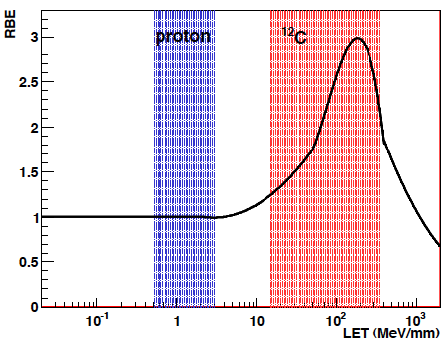
\includegraphics[width=8cm, keepaspectratio]{figs/RBE.png}
		\caption{Relative Biological Effectiveness in funzione del LET}
         \label{RBE}
\end{figure}

Ultima grandezza da definire è l'Oxygen Enhancement Ratio (OER). Gli effetti della radiazione ionizzante in generale sono amplificati dalla presenza di ossigeno. Allora può essere interessante verificare gli effetti di una certa radiazione confrontandoli in presenza di ossigeno o meno. Il rapporto tra i due casi è proprio l'OER:

\begin{equation}
\text{OER}=\frac{\text{Dose in mancanza di ossigeno}}{\text{Dose in aria}}
\end{equation}

Questo effetto varia anche con il LET, per una stessa radiazione.

\begin{figure}
\centering
		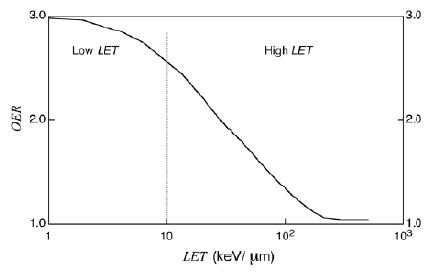
\includegraphics[width=8cm, keepaspectratio]{figs/OER.png}
		\caption{Oxygen Enhancement Ratio in funzione del LET}
         \label{OER}
\end{figure}

\section{Strumenti di Dosimetria} 

I dosimetri possono essere attivi, se misurano la loro grandezza al variare del tempo, o passivi, se sono cumulativi. Un dosimetro utile ha le seguenti proprietà:
\begin{itemize}
\item Alta accuratezza e precisione
\item Segnale lineare su un range ampio
\item Poca dipendenza in questa linearità dalla dose, dal rate di dose e dall'energia della radiazione
\item Indipendenza dalla direzione della radiazione incidente
\item Alta risoluzione spaziale
\end{itemize}

Qualunque dosimetro perde linearità tra risposta e dose effettiva. Questo può avvenire per superlinearità o per saturazione. Il primo caso può anche essere utile avendo un software che si aspetta la superlinearità e la sfrutta per aumentare la risoluzione dello strumento.

Un esempio di dosimetro è la camera a ionizzazione. Di solito è cilindrica, delle dimensioni di una penna, con armatura esterna in grafite e interna in alluminio. Il segnale elettrico si può trasformare in una lettura di Exposure. Può anche essere a pozzo, per misurare grandezze relative a sorgenti puntiformi che si mettono sopra il pozzo. Questo tipo di camere ha alta sensibilità e può funzionare in maniera attiva.

Altro tipo di rivelatore è il Film Radiografico \cite{Films}, che consiste in un coating metallico che emette elettroni per effetto fotoelettrico quando è inciso da una radiazione, i quali vanno a ionizzare la sottostante emulsione di AgBr. A questo punto l'argento si neutralizza senza legarsi di nuovo col bromo. L'argento è nero, dunque quello che osservo quando la pellicola è sottoposta a radiazione è un annerimento graduale.
Infine si illumina la pellicola e ne si osserva l'opacità, stimabile come segue:

\begin{equation}
\text{OD}=\log_{10}\left(\frac{I}{I_0}\right)
\end{equation}

L'opacità è poi una funzione monotona dell'exposure, e dunque è possibile ricavare quest'ultima grandezza.

Un Film Radiocromico invece è una pellicola contenente una tinta che polimerizza quando viene investita da radiazione e dunque mostra colore dopo essere stata colpita (GafChromic).

Altro tipo di dosimetri sono quelli che si basano su fenomeni di luminescenza quali fosforescenza e fluorescenza \cite{TLD}. Attraverso il posizionamento di impurità si creano stati metastabili intermedi nel decadimento di elettroni eccitati dalla radiazione, che dunque passando per questi stati emettono luce visibile.

Infine vi sono i detector a semiconduttore in cui la radiazione ionizzante incidente crea coppie elettrone-lacuna che generano una corrente all'interno del semiconduttore.

Per quanto riguarda la dosimetria di neutroni si usano materiali che contengono nuclei ad alta sezione d'urto con i neutroni, così che la reazione crei particelle cariche, poi facilmente tracciabili. 

Bibliografia e approfondimenti sulla dosimetria: \cite{Corvisiero2} \cite{Beringer3} \cite{Laitano}.


% !TEX root = main.tex

\chapter{Fisica dei Neutroni}

Il Neutrone è un barione di carica neutra, con spin $\frac{1}{2}$, composto dai quark $udd$, con vita media $\tau_{1/2}=889\pm 2 \ s$ e massa $m_n=1,67\cdot 10{-27} \ kg$. 
La vita media del neutrone denota che esso non è stabile quando non è legato ad altri barioni, e decade $\beta - $ creando un protone, un elettrone e un antineutrino.

Un neutrone può essere termale, se ha energia cinetica dell'ordine dei meV ed è stato prodotto per fissione, oppure può essere caldo, se ha energie più alte e deve essere stato prodotto da acceleratori o altri metodi che vedremo.

\section{Fissione Nucleare}

La fissione spontanea avviene quando in un nucleo pesante ci sono decadimenti $\beta$ o cattura elettronica. Si osserva che il decadimento di neutroni è molto più frequente di quello di protoni. Ciò è dato dal fatto che i neutroni non interagiscono elettromagneticamente ma solo forte, dunque il potenziale non presenta muri da scavalcare, e il neutrone può fondamentalmente evaporare dal nucleo. 
Notare che  il range della forza elettromagnetica è infinito, perché la massa della particella mediatrice è nulla, mentre il range della forza forte è finito e dell'ordine del femtometro, perché i mediatori dell'interazione tra nucleoni sono i pioni. La distribuzione delle energie con cui avviene la fissione spontanea è la seguente:

\begin{equation}
\frac{dN}{dE}=\sqrt{E}e^{-E/T}
\end{equation}

Un elemento spesso usato che sfrutta questo fenomeno è il $^{252}\text{Cf}$. $1 \ \mu g$ di Californio produce $2,3$ milioni di neutroni al secondo.

La Fissione indotta invece viene provocata dall'invio sul nucleo di particelle esterne (ad esempio neutroni termici). La reazione è esotermica, dunque non ho un energia di soglia del proiettile per farla avvenire. Attraverso una stima dell'energia prodotta dalla reazione posso stimare anche la vita media di tale reazione. Allora si osserva che le fissioni sono immediate, mentre per esempio i neutroni prodotti da interazioni deboli vengono prodotti sensibilmente in ritardo, prendendo infatti il nome di neutroni ritardati.

Nelle sorgenti a larga scala c'è un nocciolo di $^{235}\text{U}$ su cui un isotopo a fissione spontanea fa incidere neutroni termici. Il nocciolo fa fissione indotta ed emette neutroni molto energetici che vengono termalizzati in un moderatore (di solito acqua). Per portare un neutrone da energie del MeV a meV servono circa 30 collisioni. Poiché i neutroni non sono guidabili elettromagneticamente, per direzionarli semplicemente si scherma tutto tranne alcuni fori in cui vengono svolti gli esperimenti. Ogni foro è una beam line, alla cui fine c'è una block house in cui si svolge l'esperimento. In genere la fissione è un processo continuo, ma può essere reso pulsato mettendo uno schermo a intermittenza davanti al nocciolo.

Per una misura del numero di collisioni necessarie a portare il neutrone da energia $E_0$ a $E_f$ si stima la letargia:

\begin{equation}
\eta=\frac{1}{\xi}\ln\left[\frac{E_0}{E_f}\right]
\end{equation}

Dove $\eta$ è il numero di collisioni necessarie, mentre $\xi$ è definito come segue:

\begin{equation}
\xi=1+\frac{(A-1)^2}{2A}\ln\left(\frac{A-1}{A+1}\right)
\end{equation}

\section{Fusione Nucleare}

La fusione nucleare è una reazione ad altissimo Q. Un esempio è il seguente:

\begin{equation}
_1^2H+_1^3H \longrightarrow _2^4He+n+Energy \qquad \qquad \qquad Q=17\ MeV
\end{equation}

Il Q value viene spartito tra il neutrone, che prende 14 MeV e la particella alfa che se ne prende 3. 

Oggi si cerca di replicare la fusione sulla terra attraverso macchine come il TOKAMAK. Attraverso specifiche configurazioni di campo elettromagnetico si collima un plasma di ioni deuterio. Per ottenere la condizione di plasma servono temperature di $13,6 \ eV$, ovvero migliaia di gradi Kelvin. 

Ultimo metodo è la \emph{fusione inerziale}. Essa consiste nell'utilizzo di un guscio triziato contenente deuterio che viene bombardato con laser potentissimi. Il guscio dovrebbe quindi implodere sul deuterio causando fusione.


Altra sorgente di neutroni si ottiene bombardando un target con particelle cariche, ad esempio particelle $\alpha$. 

\section{Fotoproduzione e Spallazione}

Anche i nuclei hanno stati rotovibrazionali. Allora eccitando gli stati vibrazionali sempre di più con dei fotoni, posso arrivare a far uscire i neutroni dal range delle interazioni forti e separarli dal resto del nucleo. Così esso viene emesso con energia che dipende dall'energia di legame di quel nucleo.

I fotoni incidenti vengono prodotti dentro dei LINAC con ondulatori per sfruttare la radiazione di Brehmsstrahlung. Il processo completo si chiama Accelerator Driven Neutron Production.


La Spallazione è il processo che consiste nella produzione di neutroni tramite la collisione di protoni energetici contro un bersaglio di Tantanio.  Permette un guadagno neutronico elevato: 16 neutroni ogni protone incidente. Il protone sbatte contro un nucleo sparando alcuni nucleoni a sbattere contro altri nuclei, e così via, in un processo a cascata. Si fa anche con muoni come proiettili, esempio ISIS.

\section{Rilevazione di Neutroni}

Per rilevare una particella essa deve produrre un segnale elettrico. Nel caso in cui io voglia fare un conteggio delle particelle basta contare gli impulsi. Se voglio fare spettroscopia invece ogni impulso deve avere intensità proporzionale a tale energia.

Il neutrone è una particella neutra e dunque necessita di un meccanismo mediatore per essere rivelata. In generale si usano dei convertitori, ovvero dei materiali che presentano nuclei con cui i neutroni possono fare reazioni forti ed emettere particelle cariche in una camera a drift che raccoglie poi le particelle cariche sulle armature e produce una corrente. 

Il problema che non permette di fare spettroscopia neutronica per basse energie è che ad esempio nella reazione con l'elio-3 succede questo:

\begin{equation}
n+^3He \longrightarrow ^3H+^1H+0,764 \ MeV
\end{equation}

Ovvero con qualunque energia io mandi il neutrone ottengo in risultato sempre quei 0,764 MeV. Posso distinguere gli effetti sugli altri prodotti solo per altissime energie del neutrone.

I neutroni possono essere usati per fare spettroscopia molecolare: mandandoli con energie comparabili alle rotovibrazioni, essi interagiscono con la molecola per contatto, non elettromagneticamente. In tal modo gli stati elettronici della molecola non vengono alterati. 

\section{Utilizzo dei Neutroni}

Un utilizzo è l'analisi della conformazione di un cristallo attraverso diffrazione di Bragg. Nel processo si usano neutroni piuttosto che altre particelle cariche perché perderebbreo energia subito e non potrebbero penetrare a fondo. 
Seguono ulteriori applicazioni nello specifico:

\begin{itemize}
\item Small Angle Neutron Scattering (SANS), è uno studio delle figure di scattering di neutroni contro un determinato bersaglio che da informazioni sulla forma e le dimensioni di ciò che compone tale bersaglio.
\item Neutron Activation Analysis (NAA), Neutroni termici vengono assorbiti dal target che poi decade. Il processo può prendere ore. Se ne studiano i prodotti.
\item Neutron Stimulated Emission Computed Tomography (NSECT), Fa utilizzo di neutroni più energetici per far si che i decadimenti siano istantanei, per fare imaging direttamente.
\item Chip Irradiation. è il fenomeno per cui i neutroni energetici nei raggi cosmici possono intaccare dei chip causando perdita di dati o altri problemi. Il bombardamento dei chip con dei neutroni energetici artificiali serve a verificare la loro corretta schermatura 
prima che siano utilizzati per aerei o satelliti.
\end{itemize}

Bibliografia e approfondimenti sulle interazioni tra neutroni e materia: \cite{Corvisiero} \cite{Assay}\\

Bibliografia e approfondimenti sui rilevatori di neutroni: \cite{Beringer2} \cite{Knoll}


\printbibliography
\addcontentsline{toc}{chapter}{Bibliografia} 

%% \printglossaries
%% \addcontentsline{toc}{chapter}{Lista degli acronimi}

\listoffigures
\addcontentsline{toc}{chapter}{\listfigurename}

\listoftables
\addcontentsline{toc}{chapter}{\listtablename} 

\end{document}













